\documentclass[11pt]{article}

% Shared notes settings for Applied Machine Learning lectures (UPES).
% Keep this file free of \documentclass to allow reuse via \input.

\usepackage[utf8]{inputenc}
\usepackage[T1]{fontenc}
\usepackage{lmodern}          % scalable T1 fonts; without this pdflatex falls back
\input{glyphtounicode}        % to bitmapped EC Type 3 and the PDFs are neither
\pdfgentounicode=1            % searchable nor screen-reader friendly
\usepackage[a4paper,margin=1in]{geometry}
\usepackage{hyperref}
\usepackage{xurl}
\usepackage{booktabs}
\usepackage{amsmath}
\usepackage{amssymb}
\usepackage{listings}
\usepackage{xcolor}
\usepackage{enumitem}
\usepackage{parskip}

% Code listings (Python-oriented for this subject).
\lstset{
  language=Python,
  basicstyle=\ttfamily\small,
  keywordstyle=\color{blue},
  commentstyle=\color{gray},
  stringstyle=\color{teal},
  showstringspaces=false,
  columns=fullflexible,
  frame=single,
  framerule=0.2pt,
  breaklines=true
}

\setlist[itemize]{topsep=0.3em,itemsep=0.2em}
\setlist[enumerate]{topsep=0.3em,itemsep=0.2em}

% Simple per-section source line.
\newcommand{\notesources}[1]{\par\noindent{\small\color{gray}\textit{Sources:} \sloppy #1\par}}

% Unit-wise source strings for this subject (used by slides + notes).
% Path is relative to the lecture `latex/` folder (the compilation CWD).
\IfFileExists{../../../_shared/aml-sources.tex}{%
  % Source strings for Applied Machine Learning (CSAI2017P) — used by slides + notes.
% Prescribed texts and reference books are taken from the course syllabus.
% Support texts are the author-hosted open-access editions:
%   statlearning.com            (ISL with Python)
%   probml.github.io/pml-book   (Murphy, Probabilistic Machine Learning)
%   d2l.ai                      (Dive into Deep Learning)
%   mml-book.github.io          (Mathematics for Machine Learning)

\newcommand{\AMLRepoURL}{https://github.com/tali7c/Applied-Machine-Learning}

% --- prescribed -------------------------------------------------------------
\newcommand{\AMLPrescribed}{%
M\"uller and Guido, \textit{Introduction to Machine Learning with Python}, O'Reilly, 2016.;%
Bishop, \textit{Pattern Recognition and Machine Learning}, Springer, 2006.;%
Murphy, \textit{Machine Learning: A Probabilistic Perspective}, MIT Press, 2012.;%
Han, Kamber and Pei, \textit{Data Mining: Concepts and Techniques} (3e), Morgan Kaufmann, 2012.%
}

% --- unit-wise ---------------------------------------------------------------
\newcommand{\AMLUnitISources}{%
M\"uller and Guido, \textit{Introduction to Machine Learning with Python}, Ch. 1.;%
Bishop, \textit{Pattern Recognition and Machine Learning}, Ch. 1.;%
Murphy, \textit{Probabilistic Machine Learning: An Introduction}, MIT Press, 2022, Ch. 1.;%
Mitchell, \textit{Machine Learning}, McGraw Hill, 1997, Ch. 1.;%
Scikit-learn documentation, accessed 2026-08-04.%
}

\newcommand{\AMLUnitIISources}{%
Bishop, \textit{Pattern Recognition and Machine Learning}, \S1.5, \S4.3, \S7.1.;%
Zhang, Lipton, Li and Smola, \textit{Dive into Deep Learning}, \S3.4.;%
Shalev-Shwartz and Ben-David, \textit{Understanding Machine Learning}, Ch. 15.;%
Murphy, \textit{Probabilistic Machine Learning: An Introduction}, Ch. 5.%
}

\newcommand{\AMLUnitIIISources}{%
Zhang, Lipton, Li and Smola, \textit{Dive into Deep Learning}, Ch. 12 (Optimization Algorithms).;%
Deisenroth, Faisal and Ong, \textit{Mathematics for Machine Learning}, Ch. 7.;%
Kingma and Ba, ``Adam: A Method for Stochastic Optimization,'' ICLR 2015.;%
Ruder, ``An overview of gradient descent optimization algorithms,'' arXiv:1609.04747, 2016.%
}

\newcommand{\AMLUnitIVSources}{%
Han, Kamber and Pei, \textit{Data Mining: Concepts and Techniques} (3e), Ch. 3.;%
M\"uller and Guido, \textit{Introduction to Machine Learning with Python}, Ch. 3--4.;%
James, Witten, Hastie, Tibshirani and Taylor, \textit{An Introduction to Statistical Learning with Python}, Ch. 5--6, 12.;%
Scikit-learn documentation (preprocessing, model selection), accessed 2026-08-04.%
}

\newcommand{\AMLUnitVSources}{%
James et al., \textit{An Introduction to Statistical Learning with Python}, Ch. 3--6.;%
Bishop, \textit{Pattern Recognition and Machine Learning}, Ch. 3.;%
Deisenroth, Faisal and Ong, \textit{Mathematics for Machine Learning}, Ch. 9.;%
M\"uller and Guido, \textit{Introduction to Machine Learning with Python}, \S2.3.%
}

\newcommand{\AMLUnitVISources}{%
Han, Kamber and Pei, \textit{Data Mining: Concepts and Techniques} (3e), Ch. 8--9.;%
James et al., \textit{An Introduction to Statistical Learning with Python}, Ch. 8--9.;%
Bishop, \textit{Pattern Recognition and Machine Learning}, Ch. 4--5, 7, 14.;%
Zhang et al., \textit{Dive into Deep Learning}, Ch. 5.%
}

\newcommand{\AMLUnitVIISources}{%
Han, Kamber and Pei, \textit{Data Mining: Concepts and Techniques} (3e), Ch. 10.;%
James et al., \textit{An Introduction to Statistical Learning with Python}, Ch. 12.;%
M\"uller and Guido, \textit{Introduction to Machine Learning with Python}, \S3.5.;%
Ester, Kriegel, Sander and Xu, ``A density-based algorithm for discovering clusters (DBSCAN),'' KDD 1996.%
}

\newcommand{\AMLLabSources}{%
M\"uller and Guido, \textit{Introduction to Machine Learning with Python}, companion notebooks.;%
McKinney, \textit{Python for Data Analysis} (3e), O'Reilly, 2022.;%
Scikit-learn user guide, accessed 2026-08-04.;%
Matplotlib and Seaborn documentation, accessed 2026-08-04.%
}
%
}{%
  % Faculty copies live under `private/` so their compile CWD is different.
  \IfFileExists{../../../../public/_shared/aml-sources.tex}{%
    % Source strings for Applied Machine Learning (CSAI2017P) — used by slides + notes.
% Prescribed texts and reference books are taken from the course syllabus.
% Support texts are the author-hosted open-access editions:
%   statlearning.com            (ISL with Python)
%   probml.github.io/pml-book   (Murphy, Probabilistic Machine Learning)
%   d2l.ai                      (Dive into Deep Learning)
%   mml-book.github.io          (Mathematics for Machine Learning)

\newcommand{\AMLRepoURL}{https://github.com/tali7c/Applied-Machine-Learning}

% --- prescribed -------------------------------------------------------------
\newcommand{\AMLPrescribed}{%
M\"uller and Guido, \textit{Introduction to Machine Learning with Python}, O'Reilly, 2016.;%
Bishop, \textit{Pattern Recognition and Machine Learning}, Springer, 2006.;%
Murphy, \textit{Machine Learning: A Probabilistic Perspective}, MIT Press, 2012.;%
Han, Kamber and Pei, \textit{Data Mining: Concepts and Techniques} (3e), Morgan Kaufmann, 2012.%
}

% --- unit-wise ---------------------------------------------------------------
\newcommand{\AMLUnitISources}{%
M\"uller and Guido, \textit{Introduction to Machine Learning with Python}, Ch. 1.;%
Bishop, \textit{Pattern Recognition and Machine Learning}, Ch. 1.;%
Murphy, \textit{Probabilistic Machine Learning: An Introduction}, MIT Press, 2022, Ch. 1.;%
Mitchell, \textit{Machine Learning}, McGraw Hill, 1997, Ch. 1.;%
Scikit-learn documentation, accessed 2026-08-04.%
}

\newcommand{\AMLUnitIISources}{%
Bishop, \textit{Pattern Recognition and Machine Learning}, \S1.5, \S4.3, \S7.1.;%
Zhang, Lipton, Li and Smola, \textit{Dive into Deep Learning}, \S3.4.;%
Shalev-Shwartz and Ben-David, \textit{Understanding Machine Learning}, Ch. 15.;%
Murphy, \textit{Probabilistic Machine Learning: An Introduction}, Ch. 5.%
}

\newcommand{\AMLUnitIIISources}{%
Zhang, Lipton, Li and Smola, \textit{Dive into Deep Learning}, Ch. 12 (Optimization Algorithms).;%
Deisenroth, Faisal and Ong, \textit{Mathematics for Machine Learning}, Ch. 7.;%
Kingma and Ba, ``Adam: A Method for Stochastic Optimization,'' ICLR 2015.;%
Ruder, ``An overview of gradient descent optimization algorithms,'' arXiv:1609.04747, 2016.%
}

\newcommand{\AMLUnitIVSources}{%
Han, Kamber and Pei, \textit{Data Mining: Concepts and Techniques} (3e), Ch. 3.;%
M\"uller and Guido, \textit{Introduction to Machine Learning with Python}, Ch. 3--4.;%
James, Witten, Hastie, Tibshirani and Taylor, \textit{An Introduction to Statistical Learning with Python}, Ch. 5--6, 12.;%
Scikit-learn documentation (preprocessing, model selection), accessed 2026-08-04.%
}

\newcommand{\AMLUnitVSources}{%
James et al., \textit{An Introduction to Statistical Learning with Python}, Ch. 3--6.;%
Bishop, \textit{Pattern Recognition and Machine Learning}, Ch. 3.;%
Deisenroth, Faisal and Ong, \textit{Mathematics for Machine Learning}, Ch. 9.;%
M\"uller and Guido, \textit{Introduction to Machine Learning with Python}, \S2.3.%
}

\newcommand{\AMLUnitVISources}{%
Han, Kamber and Pei, \textit{Data Mining: Concepts and Techniques} (3e), Ch. 8--9.;%
James et al., \textit{An Introduction to Statistical Learning with Python}, Ch. 8--9.;%
Bishop, \textit{Pattern Recognition and Machine Learning}, Ch. 4--5, 7, 14.;%
Zhang et al., \textit{Dive into Deep Learning}, Ch. 5.%
}

\newcommand{\AMLUnitVIISources}{%
Han, Kamber and Pei, \textit{Data Mining: Concepts and Techniques} (3e), Ch. 10.;%
James et al., \textit{An Introduction to Statistical Learning with Python}, Ch. 12.;%
M\"uller and Guido, \textit{Introduction to Machine Learning with Python}, \S3.5.;%
Ester, Kriegel, Sander and Xu, ``A density-based algorithm for discovering clusters (DBSCAN),'' KDD 1996.%
}

\newcommand{\AMLLabSources}{%
M\"uller and Guido, \textit{Introduction to Machine Learning with Python}, companion notebooks.;%
McKinney, \textit{Python for Data Analysis} (3e), O'Reilly, 2022.;%
Scikit-learn user guide, accessed 2026-08-04.;%
Matplotlib and Seaborn documentation, accessed 2026-08-04.%
}
%
  }{%
    % Question papers live at `private/<family>/<instrument>/`.
    \IfFileExists{../../../public/_shared/aml-sources.tex}{%
      % Source strings for Applied Machine Learning (CSAI2017P) — used by slides + notes.
% Prescribed texts and reference books are taken from the course syllabus.
% Support texts are the author-hosted open-access editions:
%   statlearning.com            (ISL with Python)
%   probml.github.io/pml-book   (Murphy, Probabilistic Machine Learning)
%   d2l.ai                      (Dive into Deep Learning)
%   mml-book.github.io          (Mathematics for Machine Learning)

\newcommand{\AMLRepoURL}{https://github.com/tali7c/Applied-Machine-Learning}

% --- prescribed -------------------------------------------------------------
\newcommand{\AMLPrescribed}{%
M\"uller and Guido, \textit{Introduction to Machine Learning with Python}, O'Reilly, 2016.;%
Bishop, \textit{Pattern Recognition and Machine Learning}, Springer, 2006.;%
Murphy, \textit{Machine Learning: A Probabilistic Perspective}, MIT Press, 2012.;%
Han, Kamber and Pei, \textit{Data Mining: Concepts and Techniques} (3e), Morgan Kaufmann, 2012.%
}

% --- unit-wise ---------------------------------------------------------------
\newcommand{\AMLUnitISources}{%
M\"uller and Guido, \textit{Introduction to Machine Learning with Python}, Ch. 1.;%
Bishop, \textit{Pattern Recognition and Machine Learning}, Ch. 1.;%
Murphy, \textit{Probabilistic Machine Learning: An Introduction}, MIT Press, 2022, Ch. 1.;%
Mitchell, \textit{Machine Learning}, McGraw Hill, 1997, Ch. 1.;%
Scikit-learn documentation, accessed 2026-08-04.%
}

\newcommand{\AMLUnitIISources}{%
Bishop, \textit{Pattern Recognition and Machine Learning}, \S1.5, \S4.3, \S7.1.;%
Zhang, Lipton, Li and Smola, \textit{Dive into Deep Learning}, \S3.4.;%
Shalev-Shwartz and Ben-David, \textit{Understanding Machine Learning}, Ch. 15.;%
Murphy, \textit{Probabilistic Machine Learning: An Introduction}, Ch. 5.%
}

\newcommand{\AMLUnitIIISources}{%
Zhang, Lipton, Li and Smola, \textit{Dive into Deep Learning}, Ch. 12 (Optimization Algorithms).;%
Deisenroth, Faisal and Ong, \textit{Mathematics for Machine Learning}, Ch. 7.;%
Kingma and Ba, ``Adam: A Method for Stochastic Optimization,'' ICLR 2015.;%
Ruder, ``An overview of gradient descent optimization algorithms,'' arXiv:1609.04747, 2016.%
}

\newcommand{\AMLUnitIVSources}{%
Han, Kamber and Pei, \textit{Data Mining: Concepts and Techniques} (3e), Ch. 3.;%
M\"uller and Guido, \textit{Introduction to Machine Learning with Python}, Ch. 3--4.;%
James, Witten, Hastie, Tibshirani and Taylor, \textit{An Introduction to Statistical Learning with Python}, Ch. 5--6, 12.;%
Scikit-learn documentation (preprocessing, model selection), accessed 2026-08-04.%
}

\newcommand{\AMLUnitVSources}{%
James et al., \textit{An Introduction to Statistical Learning with Python}, Ch. 3--6.;%
Bishop, \textit{Pattern Recognition and Machine Learning}, Ch. 3.;%
Deisenroth, Faisal and Ong, \textit{Mathematics for Machine Learning}, Ch. 9.;%
M\"uller and Guido, \textit{Introduction to Machine Learning with Python}, \S2.3.%
}

\newcommand{\AMLUnitVISources}{%
Han, Kamber and Pei, \textit{Data Mining: Concepts and Techniques} (3e), Ch. 8--9.;%
James et al., \textit{An Introduction to Statistical Learning with Python}, Ch. 8--9.;%
Bishop, \textit{Pattern Recognition and Machine Learning}, Ch. 4--5, 7, 14.;%
Zhang et al., \textit{Dive into Deep Learning}, Ch. 5.%
}

\newcommand{\AMLUnitVIISources}{%
Han, Kamber and Pei, \textit{Data Mining: Concepts and Techniques} (3e), Ch. 10.;%
James et al., \textit{An Introduction to Statistical Learning with Python}, Ch. 12.;%
M\"uller and Guido, \textit{Introduction to Machine Learning with Python}, \S3.5.;%
Ester, Kriegel, Sander and Xu, ``A density-based algorithm for discovering clusters (DBSCAN),'' KDD 1996.%
}

\newcommand{\AMLLabSources}{%
M\"uller and Guido, \textit{Introduction to Machine Learning with Python}, companion notebooks.;%
McKinney, \textit{Python for Data Analysis} (3e), O'Reilly, 2022.;%
Scikit-learn user guide, accessed 2026-08-04.;%
Matplotlib and Seaborn documentation, accessed 2026-08-04.%
}
%
    }{%
      % Marking schemes live at `private/solutions/<family>/<id>/latex/`.
      \IfFileExists{../../../../../public/_shared/aml-sources.tex}{%
        % Source strings for Applied Machine Learning (CSAI2017P) — used by slides + notes.
% Prescribed texts and reference books are taken from the course syllabus.
% Support texts are the author-hosted open-access editions:
%   statlearning.com            (ISL with Python)
%   probml.github.io/pml-book   (Murphy, Probabilistic Machine Learning)
%   d2l.ai                      (Dive into Deep Learning)
%   mml-book.github.io          (Mathematics for Machine Learning)

\newcommand{\AMLRepoURL}{https://github.com/tali7c/Applied-Machine-Learning}

% --- prescribed -------------------------------------------------------------
\newcommand{\AMLPrescribed}{%
M\"uller and Guido, \textit{Introduction to Machine Learning with Python}, O'Reilly, 2016.;%
Bishop, \textit{Pattern Recognition and Machine Learning}, Springer, 2006.;%
Murphy, \textit{Machine Learning: A Probabilistic Perspective}, MIT Press, 2012.;%
Han, Kamber and Pei, \textit{Data Mining: Concepts and Techniques} (3e), Morgan Kaufmann, 2012.%
}

% --- unit-wise ---------------------------------------------------------------
\newcommand{\AMLUnitISources}{%
M\"uller and Guido, \textit{Introduction to Machine Learning with Python}, Ch. 1.;%
Bishop, \textit{Pattern Recognition and Machine Learning}, Ch. 1.;%
Murphy, \textit{Probabilistic Machine Learning: An Introduction}, MIT Press, 2022, Ch. 1.;%
Mitchell, \textit{Machine Learning}, McGraw Hill, 1997, Ch. 1.;%
Scikit-learn documentation, accessed 2026-08-04.%
}

\newcommand{\AMLUnitIISources}{%
Bishop, \textit{Pattern Recognition and Machine Learning}, \S1.5, \S4.3, \S7.1.;%
Zhang, Lipton, Li and Smola, \textit{Dive into Deep Learning}, \S3.4.;%
Shalev-Shwartz and Ben-David, \textit{Understanding Machine Learning}, Ch. 15.;%
Murphy, \textit{Probabilistic Machine Learning: An Introduction}, Ch. 5.%
}

\newcommand{\AMLUnitIIISources}{%
Zhang, Lipton, Li and Smola, \textit{Dive into Deep Learning}, Ch. 12 (Optimization Algorithms).;%
Deisenroth, Faisal and Ong, \textit{Mathematics for Machine Learning}, Ch. 7.;%
Kingma and Ba, ``Adam: A Method for Stochastic Optimization,'' ICLR 2015.;%
Ruder, ``An overview of gradient descent optimization algorithms,'' arXiv:1609.04747, 2016.%
}

\newcommand{\AMLUnitIVSources}{%
Han, Kamber and Pei, \textit{Data Mining: Concepts and Techniques} (3e), Ch. 3.;%
M\"uller and Guido, \textit{Introduction to Machine Learning with Python}, Ch. 3--4.;%
James, Witten, Hastie, Tibshirani and Taylor, \textit{An Introduction to Statistical Learning with Python}, Ch. 5--6, 12.;%
Scikit-learn documentation (preprocessing, model selection), accessed 2026-08-04.%
}

\newcommand{\AMLUnitVSources}{%
James et al., \textit{An Introduction to Statistical Learning with Python}, Ch. 3--6.;%
Bishop, \textit{Pattern Recognition and Machine Learning}, Ch. 3.;%
Deisenroth, Faisal and Ong, \textit{Mathematics for Machine Learning}, Ch. 9.;%
M\"uller and Guido, \textit{Introduction to Machine Learning with Python}, \S2.3.%
}

\newcommand{\AMLUnitVISources}{%
Han, Kamber and Pei, \textit{Data Mining: Concepts and Techniques} (3e), Ch. 8--9.;%
James et al., \textit{An Introduction to Statistical Learning with Python}, Ch. 8--9.;%
Bishop, \textit{Pattern Recognition and Machine Learning}, Ch. 4--5, 7, 14.;%
Zhang et al., \textit{Dive into Deep Learning}, Ch. 5.%
}

\newcommand{\AMLUnitVIISources}{%
Han, Kamber and Pei, \textit{Data Mining: Concepts and Techniques} (3e), Ch. 10.;%
James et al., \textit{An Introduction to Statistical Learning with Python}, Ch. 12.;%
M\"uller and Guido, \textit{Introduction to Machine Learning with Python}, \S3.5.;%
Ester, Kriegel, Sander and Xu, ``A density-based algorithm for discovering clusters (DBSCAN),'' KDD 1996.%
}

\newcommand{\AMLLabSources}{%
M\"uller and Guido, \textit{Introduction to Machine Learning with Python}, companion notebooks.;%
McKinney, \textit{Python for Data Analysis} (3e), O'Reilly, 2022.;%
Scikit-learn user guide, accessed 2026-08-04.;%
Matplotlib and Seaborn documentation, accessed 2026-08-04.%
}
%
      }{%
        % Source strings for Applied Machine Learning (CSAI2017P) — used by slides + notes.
% Prescribed texts and reference books are taken from the course syllabus.
% Support texts are the author-hosted open-access editions:
%   statlearning.com            (ISL with Python)
%   probml.github.io/pml-book   (Murphy, Probabilistic Machine Learning)
%   d2l.ai                      (Dive into Deep Learning)
%   mml-book.github.io          (Mathematics for Machine Learning)

\newcommand{\AMLRepoURL}{https://github.com/tali7c/Applied-Machine-Learning}

% --- prescribed -------------------------------------------------------------
\newcommand{\AMLPrescribed}{%
M\"uller and Guido, \textit{Introduction to Machine Learning with Python}, O'Reilly, 2016.;%
Bishop, \textit{Pattern Recognition and Machine Learning}, Springer, 2006.;%
Murphy, \textit{Machine Learning: A Probabilistic Perspective}, MIT Press, 2012.;%
Han, Kamber and Pei, \textit{Data Mining: Concepts and Techniques} (3e), Morgan Kaufmann, 2012.%
}

% --- unit-wise ---------------------------------------------------------------
\newcommand{\AMLUnitISources}{%
M\"uller and Guido, \textit{Introduction to Machine Learning with Python}, Ch. 1.;%
Bishop, \textit{Pattern Recognition and Machine Learning}, Ch. 1.;%
Murphy, \textit{Probabilistic Machine Learning: An Introduction}, MIT Press, 2022, Ch. 1.;%
Mitchell, \textit{Machine Learning}, McGraw Hill, 1997, Ch. 1.;%
Scikit-learn documentation, accessed 2026-08-04.%
}

\newcommand{\AMLUnitIISources}{%
Bishop, \textit{Pattern Recognition and Machine Learning}, \S1.5, \S4.3, \S7.1.;%
Zhang, Lipton, Li and Smola, \textit{Dive into Deep Learning}, \S3.4.;%
Shalev-Shwartz and Ben-David, \textit{Understanding Machine Learning}, Ch. 15.;%
Murphy, \textit{Probabilistic Machine Learning: An Introduction}, Ch. 5.%
}

\newcommand{\AMLUnitIIISources}{%
Zhang, Lipton, Li and Smola, \textit{Dive into Deep Learning}, Ch. 12 (Optimization Algorithms).;%
Deisenroth, Faisal and Ong, \textit{Mathematics for Machine Learning}, Ch. 7.;%
Kingma and Ba, ``Adam: A Method for Stochastic Optimization,'' ICLR 2015.;%
Ruder, ``An overview of gradient descent optimization algorithms,'' arXiv:1609.04747, 2016.%
}

\newcommand{\AMLUnitIVSources}{%
Han, Kamber and Pei, \textit{Data Mining: Concepts and Techniques} (3e), Ch. 3.;%
M\"uller and Guido, \textit{Introduction to Machine Learning with Python}, Ch. 3--4.;%
James, Witten, Hastie, Tibshirani and Taylor, \textit{An Introduction to Statistical Learning with Python}, Ch. 5--6, 12.;%
Scikit-learn documentation (preprocessing, model selection), accessed 2026-08-04.%
}

\newcommand{\AMLUnitVSources}{%
James et al., \textit{An Introduction to Statistical Learning with Python}, Ch. 3--6.;%
Bishop, \textit{Pattern Recognition and Machine Learning}, Ch. 3.;%
Deisenroth, Faisal and Ong, \textit{Mathematics for Machine Learning}, Ch. 9.;%
M\"uller and Guido, \textit{Introduction to Machine Learning with Python}, \S2.3.%
}

\newcommand{\AMLUnitVISources}{%
Han, Kamber and Pei, \textit{Data Mining: Concepts and Techniques} (3e), Ch. 8--9.;%
James et al., \textit{An Introduction to Statistical Learning with Python}, Ch. 8--9.;%
Bishop, \textit{Pattern Recognition and Machine Learning}, Ch. 4--5, 7, 14.;%
Zhang et al., \textit{Dive into Deep Learning}, Ch. 5.%
}

\newcommand{\AMLUnitVIISources}{%
Han, Kamber and Pei, \textit{Data Mining: Concepts and Techniques} (3e), Ch. 10.;%
James et al., \textit{An Introduction to Statistical Learning with Python}, Ch. 12.;%
M\"uller and Guido, \textit{Introduction to Machine Learning with Python}, \S3.5.;%
Ester, Kriegel, Sander and Xu, ``A density-based algorithm for discovering clusters (DBSCAN),'' KDD 1996.%
}

\newcommand{\AMLLabSources}{%
M\"uller and Guido, \textit{Introduction to Machine Learning with Python}, companion notebooks.;%
McKinney, \textit{Python for Data Analysis} (3e), O'Reilly, 2022.;%
Scikit-learn user guide, accessed 2026-08-04.;%
Matplotlib and Seaborn documentation, accessed 2026-08-04.%
}
%
      }%
    }%
  }%
}


\graphicspath{{../figures/}}

% This lecture pairs almost every paragraph with a listing and its output, so
% the default \medskipamount around each block adds up to several pages.
\lstset{aboveskip=3pt, belowskip=3pt}
\lstdefinestyle{amlout}{language={}, keepspaces=true,
  basicstyle=\ttfamily\footnotesize\color{black!80},
  backgroundcolor=\color{black!4}, frame=leftline, framerule=2pt,
  rulecolor=\color{black!25}, breaklines=true, columns=fullflexible,
  xleftmargin=8pt, aboveskip=2pt, belowskip=4pt, literate={-}{{-}}1}
\captionsetup{skip=4pt, font=small}
% Ten wide figures in a text-dense document: let them share pages with prose
% instead of being pushed onto float pages of their own.
\renewcommand{\topfraction}{0.92}
\renewcommand{\bottomfraction}{0.75}
\renewcommand{\textfraction}{0.06}
\renewcommand{\floatpagefraction}{0.85}
\setlength{\floatsep}{6pt plus 2pt minus 2pt}
\setlength{\textfloatsep}{8pt plus 2pt minus 2pt}
\setlength{\intextsep}{8pt plus 2pt minus 2pt}

\newcommand{\TP}{\mathrm{TP}}
\newcommand{\FP}{\mathrm{FP}}
\newcommand{\TN}{\mathrm{TN}}
\newcommand{\FN}{\mathrm{FN}}
\newcommand{\TPR}{\mathrm{TPR}}
\newcommand{\FPR}{\mathrm{FPR}}

\title{Applied Machine Learning\\Unit 06 --- Lecture 19 Notes\\
       Classification Model Evaluation: ROC and AUC}
\author{Tofik Ali}
\date{Autumn 2026}

\begin{document}
\maketitle

\begin{keyidea}[Read this first]
These notes are written so that you can learn the material \emph{without}
having been in the lecture. Every concept is developed from scratch, every
number you see was produced by running the code shown beside it, and every
figure was generated from real computation rather than drawn by hand.

Unit VI has given you six ways to build a classifier: nearest neighbours,
decision trees, Bayesian classifiers, ensembles, neural networks and support
vector machines. It has not yet given you a defensible way to say which one to
use. That is this lecture, and it is the last one in the unit for exactly that
reason.

The argument runs in one line. \textbf{A classifier does not output a class ---
it outputs a score, and a threshold turns that score into a class.} Accuracy,
precision, recall and F1 all describe one threshold. The ROC curve describes
\emph{all} of them at once, and the area under it, the AUC, is a single number
that turns out to have a startlingly concrete meaning: the probability that a
randomly chosen positive is scored above a randomly chosen negative.

Three results to carry out of the lecture. First, on a table with $1\%$
positives, a model that always answers ``negative'' scores $\mathbf{0.9900}$
accuracy and a useful model scores $\mathbf{0.9897}$ --- the useful one is
\emph{worse} by that measure. Second, on that same problem the ROC curve
reports an encouraging AUC of $\mathbf{0.9200}$ while the precision--recall
curve reports an average precision of $\mathbf{0.1702}$; at $90\%$ recall one
alert in twenty-two is real. Third, on \texttt{breast\_cancer} the best and
second-best of seven classifiers differ by $\mathbf{0.0003}$ of AUC while the
fold-to-fold spread is $\mathbf{0.0058}$ --- so there is no best model, and
saying there is would be an error of the same kind as reading a ruler to the
nearest micron.

Section~\ref{sec:rochand} is the centre of the lecture. Build that ROC curve
on paper before you read the code.
\end{keyidea}

\tableofcontents
\medskip

% =========================================================================
\section{How to use these notes}
\label{sec:how}

Read in order. Section~\ref{sec:auc} assumes the hand-built curve of
Section~\ref{sec:rochand}; Section~\ref{sec:rocpr} assumes both. The material
is arithmetically light --- there is no calculus in this lecture and only one
piece of probability --- but it is arithmetically \emph{dense}, and the way to
learn it is to do the small tables by hand rather than read them.

There are four kinds of box. \textbf{Key idea} --- the one sentence to remember
a month from now. \textbf{Worked example} --- a calculation done by hand, with
small numbers, before any library is used. \textbf{Caution} --- the specific
mistake that section exists to prevent. \textbf{Try it yourself} --- something
to run, with the expected output given so you can check.

Code appears in a framed block, and directly beneath it a shaded block showing
what that code \emph{actually printed}. If you run it and get something
different, trust your machine and tell me.

\subsection{What you need}

\begin{lstlisting}
pip install numpy scipy scikit-learn matplotlib
\end{lstlisting}

Every number in these notes was produced with:

\begin{lstlisting}
import numpy, scipy, sklearn, matplotlib
print("numpy", numpy.__version__, "| scipy", scipy.__version__,
      "| sklearn", sklearn.__version__,
      "| matplotlib", matplotlib.__version__)
\end{lstlisting}
\begin{codeout}
numpy 2.2.6 | scipy 1.15.3 | sklearn 1.7.2 | matplotlib 3.10.9
\end{codeout}

Three bundled datasets and one synthetic problem recur, and \textbf{none of
them downloads anything}.

\begin{lstlisting}
from sklearn.datasets import (load_breast_cancer, load_wine, load_digits,
                              make_classification)
bc   = load_breast_cancer(); Xb, yb = bc.data, bc.target
wine = load_wine();          Xw, yw = wine.data, wine.target
dg   = load_digits();        Xg, yg = dg.data, dg.target
\end{lstlisting}
\begin{codeout}
load_breast_cancer  569 rows x 30 features, classes [212 357]
load_wine           178 rows x 13 features, classes [59 71 48]
load_digits        1797 rows x 64 features, classes [178 182 177 183 181 182 181 179 174 180]
breast_cancer target names: ['malignant', 'benign']
label 1 = 'benign' is the positive class by default: prevalence 0.6274
\end{codeout}

That last line matters more than it looks. In \texttt{load\_breast\_cancer} the
label $1$ is \emph{benign}, so scikit-learn's default ``positive class'' is the
harmless one. Every metric in this lecture is asymmetric between the classes,
so before you compute anything, decide which class is positive and say so out
loud.

\begin{keyidea}[One seed, and the two kinds of number that are not it]
Everything arbitrary in these notes uses \textbf{one seed, $0$}: every
\texttt{train\_test\_split}, every subsample of the negatives, the coin-flip
scores of Section~\ref{sec:auc}, and every estimator's \texttt{random\_state}
are \texttt{random\_state=0} or \texttt{np.random.default\_rng(0)}. Every
listing that samples or shuffles shows it.

Two other things look like the same seed and are not.
\begin{itemize}
  \item \textbf{A seed that defines a dataset.} The
    \texttt{random\_state} inside \texttt{make\_classification} fixes the
    $99\!:\!1$ problem above ($0$) and the three-class problem of
    Section~\ref{sec:multi} ($1$). Change either and you have different data,
    not a different experiment, so they never move.
  \item \textbf{A sweep.} Section~\ref{sec:selection} scores every model over
    $5 \times 4 = 20$ folds, and the \emph{spread} between those folds is the
    argument of that section --- it is what tells you a gap of $0.002$ means
    nothing. So the folds stay a sweep; they are simply generated from seed
    $0$, so the spread is the same spread every time you run it.
\end{itemize}

So every number printed in these notes reproduces exactly if you run the code
as written on the library versions above --- including the ones whose whole
purpose is to vary.
\end{keyidea}

\subsection{Learning outcomes}

This lecture serves \textbf{CO3}: \emph{analyse the performance of machine
learning models and interpret the results}. By the end of it you should be able
to:

\begin{enumerate}[leftmargin=*]
  \item build a confusion matrix from a list of actual and predicted labels,
    and compute accuracy, precision, recall, sensitivity, specificity, the
    false positive rate and F1 from it, by hand;
  \item explain, with a number, why accuracy is the wrong summary when the
    classes are imbalanced;
  \item construct an ROC curve from a list of scored examples by sweeping the
    threshold, plot the staircase, and reproduce it with
    \texttt{sklearn.metrics.roc\_curve};
  \item compute AUC two ways --- as a trapezoidal area and as the probability
    that a random positive outranks a random negative --- and show that they
    agree;
  \item state what an AUC of $0.5$, an AUC below $0.5$, and AUC's invariance to
    the threshold and to the class balance mean;
  \item say when a precision--recall curve should be reported instead of, or
    alongside, an ROC curve, and justify it from the prevalence;
  \item choose a decision threshold from a stated cost ratio, and explain what
    changes when a false negative costs ten times a false positive;
  \item compute micro, macro and weighted averages for a multiclass problem by
    hand and say which one to report;
  \item compare several classifiers by cross-validated AUC with error bars, and
    judge whether an observed difference is a difference at all.
\end{enumerate}

\notesources{\AMLUnitVISources}

% =========================================================================
\section{The question, and why accuracy does not answer it}
\label{sec:whynot}

\subsection{Where we are}

Unit VI built classifiers. Lecture~13 built one from distances, Lecture~14 from
splits on attributes, Lecture~15 from Bayes' rule, Lecture~16 from votes among
many trees, Lecture~17 from layers of weights, Lecture~18 from a margin. Each of
those lectures ended with a number --- an accuracy on a held-out split --- and
each time we treated that number as though it settled something.

It does not. Two questions were left open, and they are the same question in
different clothes:

\begin{enumerate}[leftmargin=*]
  \item \textbf{Is this model any good?} A single accuracy is meaningless
    without knowing what a useless model would score.
  \item \textbf{Is this model better than that one?} A single accuracy from a
    single split has a standard error you have not measured.
\end{enumerate}

\begin{keyidea}
Evaluation is not the last chapter of the modelling story. It is the part that
decides which story you tell. If you cannot say what a useless model scores on
your problem, you cannot say whether your model is useful.
\end{keyidea}

\subsection{Accuracy, and the one situation in which it lies}

Accuracy is the fraction of predictions that were right. It is the natural
thing to compute and it is right to compute it --- but it is a \emph{weighted}
summary, and the weights are the class frequencies. When one class is rare,
accuracy is almost entirely a report on the common class.

Here is the demonstration. A synthetic problem with $20{,}000$ rows and a
$99\!:\!1$ class ratio: $200$ positives against $19{,}800$ negatives, six
informative features, moderate separation.

\begin{lstlisting}
from sklearn.datasets import make_classification
from sklearn.model_selection import train_test_split
from sklearn.dummy import DummyClassifier
from sklearn.metrics import (accuracy_score, confusion_matrix,
                             precision_score, recall_score, f1_score)

Xi, yi = make_classification(n_samples=20000, n_features=25,
                             n_informative=6, n_redundant=3,
                             weights=[0.99, 0.01], flip_y=0.0,
                             class_sep=0.9, random_state=0)  # fixes the data
Xi_tr, Xi_te, yi_tr, yi_te = train_test_split(
    Xi, yi, test_size=0.3, stratify=yi, random_state=0)   # the one seed

dumb = DummyClassifier(strategy="constant", constant=0).fit(Xi_tr, yi_tr)
pd_ = dumb.predict(Xi_te)
print("accuracy", accuracy_score(yi_te, pd_))
print(confusion_matrix(yi_te, pd_))
print("precision", precision_score(yi_te, pd_, zero_division=0),
      "recall", recall_score(yi_te, pd_, zero_division=0))
\end{lstlisting}
\begin{codeout}
rows 20000   positives 200   negatives 19800   prevalence 0.0100

A model that always answers 'negative', on the 6000 held-out rows:
  accuracy  0.9900
  confusion matrix
[[5940    0]
 [  60    0]]
  precision 0.0000   recall 0.0000   F1 0.0000
  it found 0 of the 60 positives
\end{codeout}

A model that has not looked at a single feature scores $99\%$. Write that
number on a slide and it reads as a triumph.

Now fit something real.

\begin{lstlisting}
from sklearn.pipeline import make_pipeline
from sklearn.preprocessing import StandardScaler
from sklearn.linear_model import LogisticRegression
from sklearn.metrics import roc_auc_score, average_precision_score

lr = make_pipeline(StandardScaler(),
                   LogisticRegression(max_iter=5000)).fit(Xi_tr, yi_tr)
pi = lr.predict(Xi_te)
si = lr.predict_proba(Xi_te)[:, 1]
\end{lstlisting}
\begin{codeout}
An actual logistic regression on the same split:
  accuracy  0.9897  (the constant model got 0.9900)
  accuracy gained over the constant model: -0.0003
  precision 0.3333   recall 0.0333   F1 0.0606
  it predicted 'positive' 6 times and was right 2 times
  ROC AUC   0.9200   average precision 0.1702
The useful model scores LOWER accuracy than the useless one.
\end{codeout}

\begin{caution}[The result that should stop you]
The logistic regression is \textbf{worse than the constant model by accuracy}
($0.9897$ against $0.9900$) and its ROC AUC is $0.9200$ against the constant
model's $0.5000$. Accuracy and AUC do not merely differ here; they \emph{rank
the two models in opposite orders}. If you report accuracy on an imbalanced
problem you will throw away the model that works.
\end{caution}

Two things rescue us. The first is to stop looking at a single number and look
at the four numbers underneath it --- the confusion matrix, Section~\ref{sec:cm}.
The second is to stop looking at a single \emph{threshold}, which is
Section~\ref{sec:scores} onwards.

\begin{figure}[htbp]
\centering
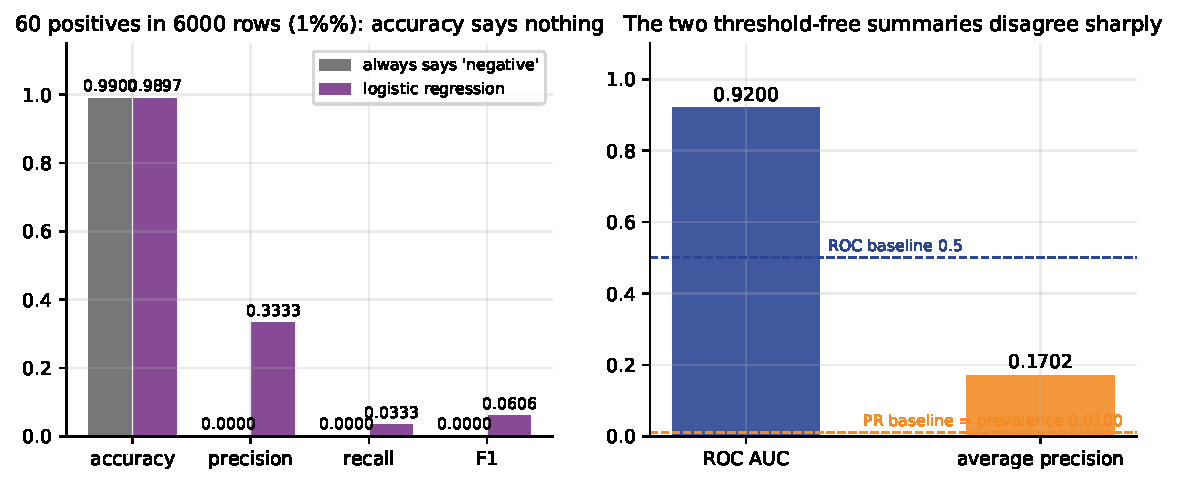
\includegraphics[width=\textwidth]{l19-imbalance-accuracy.pdf}
\caption{Left: four metrics for the constant model and for logistic regression
on the $99\!:\!1$ problem. Accuracy is indistinguishable; precision and recall
are not. Right: the two threshold-free summaries of the \emph{same} logistic
regression, each against its own baseline. They disagree, and
Section~\ref{sec:rocpr} explains why.}
\label{fig:imbalance}
\end{figure}

% =========================================================================
\section{The confusion matrix, and everything that comes out of it}
\label{sec:cm}

\subsection{Four numbers}

Fix a positive class. Every prediction on a labelled row falls into exactly one
of four boxes:

\begin{center}
\small
\begin{tabular}{@{}llll@{}}
\toprule
 & predicted negative & predicted positive & row total\\
\midrule
actually negative & $\TN$ true negative  & $\FP$ false positive & $N = \FP + \TN$\\
actually positive & $\FN$ false negative & $\TP$ true positive  & $P = \TP + \FN$\\
\bottomrule
\end{tabular}
\end{center}

The naming rule is worth stating once, because students reverse it every year:
\textbf{the second word is what the model said, the first word is whether it was
right}. A false positive is a row the model called positive and was wrong about.

\begin{worked}[Twenty patients, by hand]
Twenty people are screened. Ten of them have the disease (label $1$), ten do
not (label $0$). The model says ``disease'' for six of the ten who have it, and
for two of the ten who do not.

\smallskip
\begin{center}\footnotesize
\begin{tabular}{@{}lrrrrrrrrrr@{}}
\toprule
patient  & 1&2&3&4&5&6&7&8&9&10\\
actual   & 1&1&1&1&1&1&1&1&1&1\\
predicted& 1&1&1&1&1&1&0&0&0&0\\
cell     & TP&TP&TP&TP&TP&TP&FN&FN&FN&FN\\
\midrule
patient  & 11&12&13&14&15&16&17&18&19&20\\
actual   & 0&0&0&0&0&0&0&0&0&0\\
predicted& 1&1&0&0&0&0&0&0&0&0\\
cell     & FP&FP&TN&TN&TN&TN&TN&TN&TN&TN\\
\bottomrule
\end{tabular}
\end{center}
\smallskip

Count: $\TP = 6$, $\FN = 4$, $\FP = 2$, $\TN = 8$. Hence $P = 10$ and $N = 10$.
Now every metric in this lecture, arithmetically:
\begin{align*}
\text{accuracy} &= \frac{\TP + \TN}{P + N} = \frac{6+8}{20} = 0.7000\\[2pt]
\text{precision} &= \frac{\TP}{\TP + \FP} = \frac{6}{8} = 0.7500\\[2pt]
\text{recall} = \text{sensitivity} = \TPR &= \frac{\TP}{P} = \frac{6}{10} = 0.6000\\[2pt]
\text{specificity} &= \frac{\TN}{N} = \frac{8}{10} = 0.8000\\[2pt]
\FPR &= \frac{\FP}{N} = \frac{2}{10} = 0.2000 \;=\; 1 - \text{specificity}\\[2pt]
F_1 &= \frac{2 \cdot \text{precision} \cdot \text{recall}}
             {\text{precision} + \text{recall}}
     = \frac{2 \times 0.75 \times 0.60}{1.35} = \frac{0.9}{1.35} = 0.6667
\end{align*}
Six numbers, all from the same four counts. Nothing else is going on.
\end{worked}

Verifying with the library, on exactly those twenty rows:

\begin{lstlisting}
import numpy as np
from sklearn.metrics import confusion_matrix, classification_report

y_true = np.array([1]*10 + [0]*10)
y_pred = np.array([1]*6 + [0]*4 + [1]*2 + [0]*8)
print(confusion_matrix(y_true, y_pred))
print(classification_report(y_true, y_pred, digits=4,
      target_names=["healthy (0)", "disease (1)"]))
\end{lstlisting}
\begin{codeout}
confusion_matrix(y_true, y_pred) =
[[8 2]
 [4 6]]
rows = actual, cols = predicted, label order [0, 1]
so cm[1,1]=TP=6  cm[0,1]=FP=2  cm[1,0]=FN=4  cm[0,0]=TN=8

              precision    recall  f1-score   support

 healthy (0)     0.6667    0.8000    0.7273        10
 disease (1)     0.7500    0.6000    0.6667        10

    accuracy                         0.7000        20
   macro avg     0.7083    0.7000    0.6970        20
weighted avg     0.7083    0.7000    0.6970        20
\end{codeout}

Every hand number appears. Note that \texttt{classification\_report} gives a row
for \emph{each} class, and that the ``healthy'' row's recall $0.8000$ is what we
called specificity. Precision and recall of the negative class are specificity's
two relatives; the report gives you all of them.

\begin{caution}[The layout that catches everybody]
\texttt{confusion\_matrix} puts \textbf{actual on the rows, predicted on the
columns}, with labels in sorted order. So the top-left cell is $\TN$ and the
bottom-right is $\TP$ --- the transpose of the layout in Han, Kamber and Pei
$\S8.5.1$, and the transpose of the layout most textbooks draw. Print the matrix
and check one cell against a count you did yourself before you believe any
number derived from it.
\end{caution}

\begin{figure}[htbp]
\centering
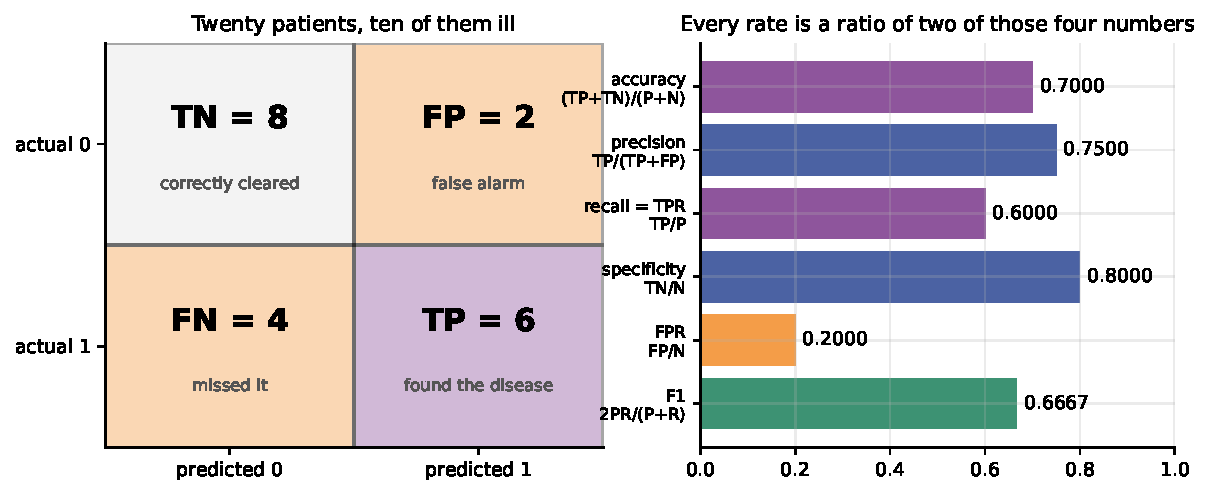
\includegraphics[width=\textwidth]{l19-confusion-matrix.pdf}
\caption{The twenty patients as four counts, and the six rates that come out of
them. Every bar on the right is a ratio of two of the four numbers on the left.}
\label{fig:cm}
\end{figure}

\subsection{Reading the four ratios}

The four counts admit many ratios; four of them matter, and they pair up.

\begin{center}\small
\begin{tabular}{@{}llll@{}}
\toprule
name & formula & denominator is & answers\\
\midrule
recall / sensitivity / $\TPR$ & $\TP/P$ & the actual positives & of the ill, how many did we find?\\
specificity / $\mathrm{TNR}$ & $\TN/N$ & the actual negatives & of the well, how many did we clear?\\
$\FPR$ & $\FP/N$ & the actual negatives & of the well, how many did we alarm?\\
precision / PPV & $\TP/(\TP+\FP)$ & the \emph{predicted} positives & of our alarms, how many were real?\\
\bottomrule
\end{tabular}
\end{center}

Two of these read down the columns of truth (recall, specificity, $\FPR$) and
one reads down a column of \emph{prediction} (precision). That single difference
is the whole of Section~\ref{sec:rocpr}, so hold on to it:

\begin{keyidea}
Recall and $\FPR$ have the class sizes in the denominator, so they do not change
when you change how many negatives you happen to have collected. Precision has
$\TP + \FP$ in the denominator, which is a quantity the \emph{prevalence}
controls. That is why the ROC curve is blind to imbalance and the
precision--recall curve is not.
\end{keyidea}

\subsection{Why $F_1$ is a harmonic mean}

$F_1$ combines precision and recall. It uses the harmonic mean, not the
arithmetic one, and the reason is a property you can check in one line: the
harmonic mean is dominated by the smaller of the two. With precision $1.0$ and
recall $0.02$ --- a model that fires almost never but is always right when it
does --- the arithmetic mean is $0.51$ and the harmonic mean is $0.0392$. The
first flatters, the second reports.

\begin{tryit}
Compute both means for $(p, r) = (1.0, 0.02)$, $(0.6, 0.6)$ and $(0.9, 0.3)$.
You should get arithmetic $0.510, 0.600, 0.600$ and harmonic
$0.0392, 0.600, 0.450$. Notice that the two $0.600$ arithmetic means describe
completely different models and the harmonic means separate them.
\end{tryit}

The general form is $F_\beta$, which weights recall $\beta$ times as heavily as
precision:
\begin{equation}
F_\beta = (1 + \beta^2)\,
  \frac{\text{precision} \times \text{recall}}
       {\beta^2 \times \text{precision} + \text{recall}} .
\label{eq:fbeta}
\end{equation}
$F_1$ is $\beta = 1$. $F_2$ is the choice when a miss hurts more than a false
alarm, and it is the first of several places in this lecture where a
\emph{business} decision enters the arithmetic.

% =========================================================================
\section{Scores, not labels}
\label{sec:scores}

Everything in Section~\ref{sec:cm} describes one confusion matrix, and a
confusion matrix requires hard labels. But a classifier does not naturally
produce hard labels. It produces a score, and \texttt{predict} applies a
threshold you never chose:

\begin{center}\small
\begin{tabular}{@{}lll@{}}
\toprule
model & score & default rule \\
\midrule
\texttt{LogisticRegression} & \texttt{predict\_proba(X)[:, 1]} & positive if $\ge 0.5$\\
\texttt{RandomForestClassifier} & \texttt{predict\_proba(X)[:, 1]} & positive if $\ge 0.5$\\
\texttt{GaussianNB} & \texttt{predict\_proba(X)[:, 1]} & positive if $\ge 0.5$\\
\texttt{KNeighborsClassifier} & fraction of the $k$ neighbours & positive if $\ge 0.5$\\
\texttt{SVC} & \texttt{decision\_function(X)} & positive if $\ge 0$\\
\texttt{MLPClassifier} & \texttt{predict\_proba(X)[:, 1]} & positive if $\ge 0.5$\\
\bottomrule
\end{tabular}
\end{center}

For the rest of this lecture we use a deliberately \emph{imperfect} model, so
that the choice of threshold has visible consequences: logistic regression on
three of the thirty \texttt{breast\_cancer} columns.

\begin{lstlisting}
COLS = [0, 1, 4]     # mean radius, mean texture, mean smoothness
Xb_tr, Xb_te, yb_tr, yb_te = train_test_split(
    Xb[:, COLS], yb, test_size=0.3, stratify=yb, random_state=0)
clf = make_pipeline(StandardScaler(),
                    LogisticRegression(max_iter=5000)).fit(Xb_tr, yb_tr)
sb = clf.predict_proba(Xb_te)[:, 1]
\end{lstlisting}
\begin{codeout}
features used: ['mean radius', 'mean texture', 'mean smoothness']
held-out rows 171   benign (positive) 107   malignant 64
ROC AUC 0.9661   accuracy at 0.5 0.9064
for comparison, the same split with all 30 features: ROC AUC 0.9956
we use the three-feature model from here on: a near-perfect model
makes every threshold look equally good, which teaches nothing.
\end{codeout}

Now sweep the threshold on that one fixed set of scores.

\begin{lstlisting}
for t in [0.05, 0.20, 0.35, 0.50, 0.65, 0.80, 0.95]:
    p = (sb >= t).astype(int)
    print(t, accuracy_score(yb_te, p), precision_score(yb_te, p),
          recall_score(yb_te, p), f1_score(yb_te, p))
print("ROC AUC", roc_auc_score(yb_te, sb))
\end{lstlisting}
\begin{codeout}
one set of scores, one AUC, many thresholds
threshold  TP  FP  FN  TN  accuracy  precision  recall     F1
   0.05    107  28   0  36    0.8363     0.7926  1.0000  0.8843
   0.20    107  19   0  45    0.8889     0.8492  1.0000  0.9185
   0.35    106  13   1  51    0.9181     0.8908  0.9907  0.9381
   0.50    100   9   7  55    0.9064     0.9174  0.9346  0.9259
   0.65     94   4  13  60    0.9006     0.9592  0.8785  0.9171
   0.80     86   4  21  60    0.8538     0.9556  0.8037  0.8731
   0.95     58   0  49  64    0.7135     1.0000  0.5421  0.7030
ROC AUC, for every row above:  0.9661
AUC is a property of the scores. The threshold is a separate decision.
\end{codeout}

\begin{keyidea}
One model, one set of scores, seven confusion matrices. Accuracy ranges over
$0.71$ to $0.92$ and F1 over $0.70$ to $0.94$, all from the same fitted model.
\textbf{Quoting a single accuracy is quoting a model \emph{and} an unstated
threshold as though they were one thing.}
\end{keyidea}

Read the table down the precision and recall columns and you see the trade that
runs through the whole lecture. Lower the threshold and you catch more positives
(recall rises to $1.0000$) at the price of more false alarms (precision falls to
$0.7926$). Raise it and the reverse. There is no threshold at which both improve,
because raising the threshold can only move rows from ``predicted positive'' to
``predicted negative''.

\begin{figure}[htbp]
\centering
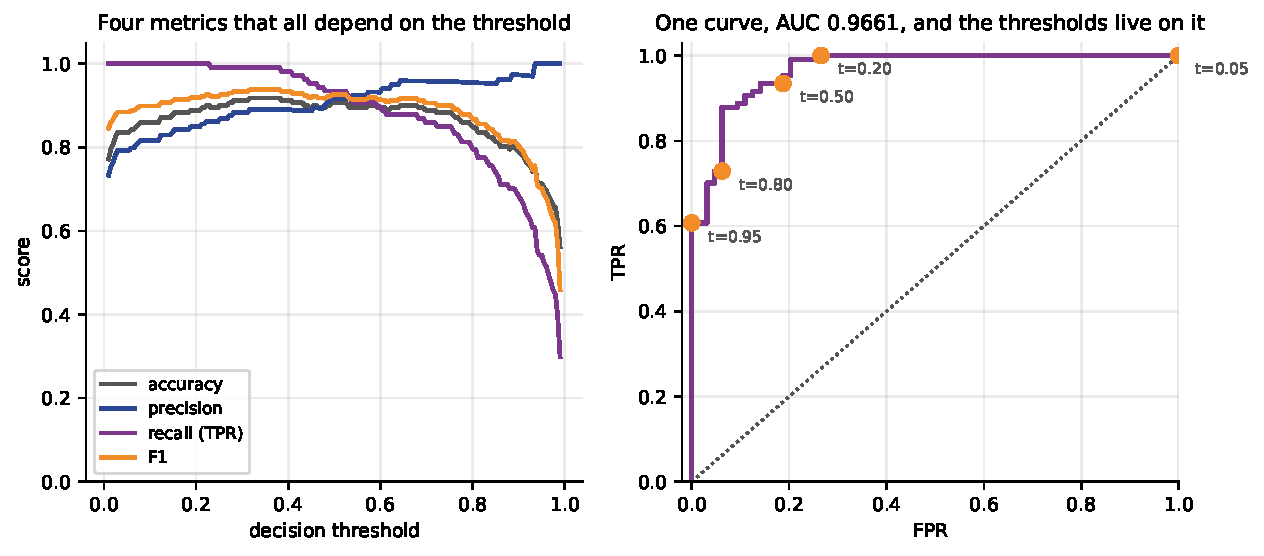
\includegraphics[width=\textwidth]{l19-threshold-sweep.pdf}
\caption{Left: the four threshold-dependent metrics as continuous functions of
the threshold, on the three-feature \texttt{breast\_cancer} model. Right: the
same information as a single curve. Each labelled point is one row of the table
above; the curve is every threshold at once.}
\label{fig:sweep}
\end{figure}

% =========================================================================
\section{Building an ROC curve by hand}
\label{sec:rochand}

This is the section the lecture exists for. Do it on paper.

\subsection{Ten scored examples}

Take ten rows: five positive, five negative, each with a score between $0$ and
$1$. Sort them by score, highest first.

\begin{center}\small
\begin{tabular}{@{}rrrrrrrrrrr@{}}
\toprule
rank  & 1 & 2 & 3 & 4 & 5 & 6 & 7 & 8 & 9 & 10\\
label & POS & POS & neg & POS & POS & neg & neg & POS & neg & neg\\
score & $0.95$ & $0.90$ & $0.85$ & $0.75$ & $0.60$ & $0.55$ & $0.45$ & $0.35$ & $0.25$ & $0.10$\\
\bottomrule
\end{tabular}
\end{center}

There are $P = 5$ positives and $N = 5$ negatives. The model is not perfect ---
a negative sits at rank $3$, above two positives --- but it is clearly better
than nothing.

\subsection{The sweep}

The recipe is mechanical. Start with the threshold above every score, so nothing
is predicted positive: $\TP = 0$, $\FP = 0$, and the point is $(0,0)$. Now lower
the threshold to each score in turn. Each time you cross a \textbf{positive}, one
row moves from $\FN$ to $\TP$, so $\TPR$ rises by $1/P = 0.2$ and $\FPR$ does not
move --- a step \emph{up}. Each time you cross a \textbf{negative}, $\FPR$ rises
by $1/N = 0.2$ and $\TPR$ does not move --- a step \emph{right}.

\begin{worked}[The whole sweep, ten rows]
\begin{center}\footnotesize
\begin{tabular}{@{}lrrrrrr@{}}
\toprule
threshold & $\TP$ & $\FP$ & $\FN$ & $\TN$ & $\FPR = \FP/5$ & $\TPR = \TP/5$\\
\midrule
(nothing predicted) & 0 & 0 & 5 & 5 & $0.0$ & $0.0$\\
$0.95$ \;(POS) & 1 & 0 & 4 & 5 & $0.0$ & $0.2$\\
$0.90$ \;(POS) & 2 & 0 & 3 & 5 & $0.0$ & $0.4$\\
$0.85$ \;(neg) & 2 & 1 & 3 & 4 & $0.2$ & $0.4$\\
$0.75$ \;(POS) & 3 & 1 & 2 & 4 & $0.2$ & $0.6$\\
$0.60$ \;(POS) & 4 & 1 & 1 & 4 & $0.2$ & $0.8$\\
$0.55$ \;(neg) & 4 & 2 & 1 & 3 & $0.4$ & $0.8$\\
$0.45$ \;(neg) & 4 & 3 & 1 & 2 & $0.6$ & $0.8$\\
$0.35$ \;(POS) & 5 & 3 & 0 & 2 & $0.6$ & $1.0$\\
$0.25$ \;(neg) & 5 & 4 & 0 & 1 & $0.8$ & $1.0$\\
$0.10$ \;(neg) & 5 & 5 & 0 & 0 & $1.0$ & $1.0$\\
\bottomrule
\end{tabular}
\end{center}
Plot the eleven $(\FPR, \TPR)$ pairs and join them with horizontal and vertical
segments. That staircase is the ROC curve. Note the two guaranteed endpoints:
$(0,0)$ when nothing is predicted positive, $(1,1)$ when everything is. Every
ROC curve you will ever see runs between those two corners.
\end{worked}

That table \emph{is} the ROC curve. Nothing has been fitted, smoothed or
estimated; it is bookkeeping on a sorted list.

\begin{keyidea}
An ROC curve is what you get when you refuse to choose a threshold and plot all
of them. Sort by score; walk down the list; step up for a positive, right for a
negative. The curve depends only on the \textbf{order} of the scores, not on
their values --- which is why any monotone rescaling of the scores leaves it
untouched.
\end{keyidea}

\subsection{The same curve from scikit-learn}

\begin{lstlisting}
from sklearn.metrics import roc_curve, auc, roc_auc_score
y10 = np.array([1, 1, 0, 1, 1, 0, 0, 1, 0, 0])
s10 = np.array([0.95, 0.90, 0.85, 0.75, 0.60, 0.55, 0.45, 0.35, 0.25, 0.10])
fpr, tpr, thr = roc_curve(y10, s10, drop_intermediate=False)
for t, f, r in zip(thr, fpr, tpr):
    print(t, f, r)
\end{lstlisting}
\begin{codeout}
sklearn roc_curve(y, s, drop_intermediate=False)
 threshold      FPR     TPR
       inf  0.0000  0.0000
      0.95  0.0000  0.2000
      0.90  0.0000  0.4000
      0.85  0.2000  0.4000
      0.75  0.2000  0.6000
      0.60  0.2000  0.8000
      0.55  0.4000  0.8000
      0.45  0.6000  0.8000
      0.35  0.6000  1.0000
      0.25  0.8000  1.0000
      0.10  1.0000  1.0000
the first threshold is np.inf: the 'predict nothing' corner (0,0).
every other row matches the hand sweep exactly.

with the default drop_intermediate=True sklearn keeps only the corners:
  8 points instead of 11, same curve, same area 0.8000
\end{codeout}

Row for row, identical to the hand table. Two details:

\begin{itemize}[leftmargin=*]
  \item The first threshold is \texttt{np.inf}. Older versions of scikit-learn
    reported \texttt{max(score) + 1} here; either way it means ``a threshold
    above everything'', the $(0,0)$ corner.
  \item By default \texttt{roc\_curve} sets \texttt{drop\_intermediate=True} and
    discards points that lie on a straight segment of the curve --- $11$ points
    become $8$. The curve and the area are unchanged. Pass
    \texttt{drop\_intermediate=False} when you are checking against a hand
    calculation, and leave the default alone when you are plotting a curve from
    thousands of rows.
\end{itemize}

\begin{figure}[htbp]
\centering
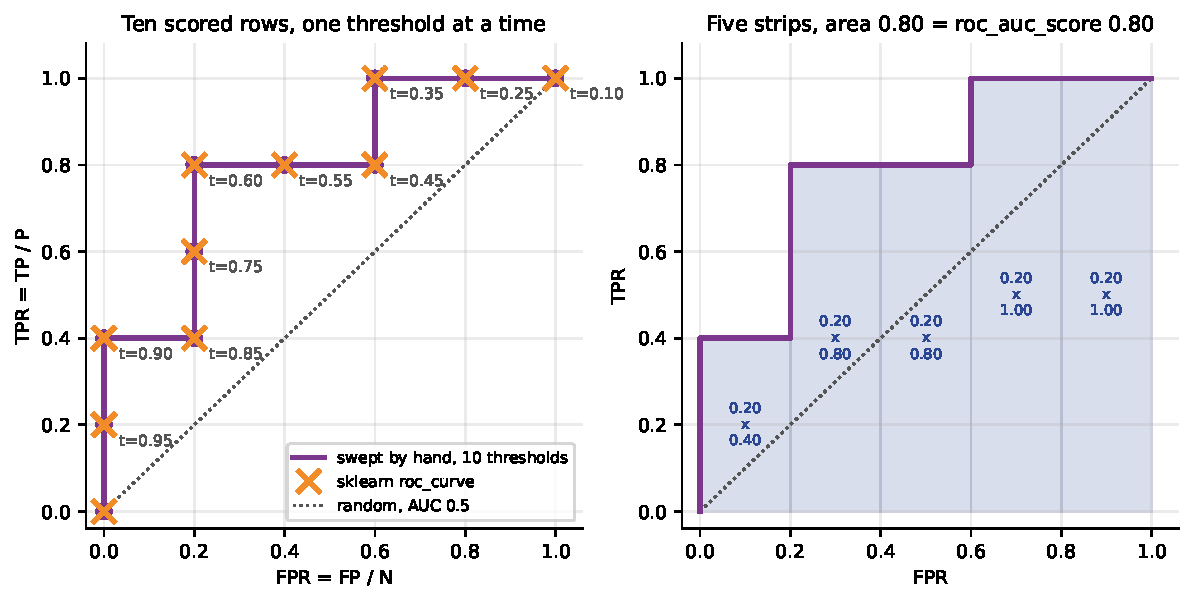
\includegraphics[width=\textwidth]{l19-roc-by-hand.pdf}
\caption{Left: the hand-swept staircase (purple, with the threshold at each
step) and \texttt{roc\_curve}'s output (orange crosses) on the same ten rows.
The largest disagreement is $0.00$. Right: the same staircase cut into five
vertical strips whose areas sum to the AUC.}
\label{fig:rochand}
\end{figure}

\subsection{Reading a curve}

Four things to look for, and they are all visible in Figure~\ref{fig:rochand}.

\begin{itemize}[leftmargin=*]
  \item \textbf{The top-left corner $(0,1)$} is the perfect classifier: every
    positive scored above every negative, so there is a threshold that catches
    all of them and alarms on none. Curves closer to that corner are better.
  \item \textbf{The diagonal} is a classifier whose scores carry no information
    about the label. It is not a line anyone draws; it is what you measure.
    Section~\ref{sec:auc} demonstrates it on coin flips.
  \item \textbf{Steepness at the left} matters most in practice. That is the
    region of high thresholds, where you fire few alarms; if you can only act on
    twenty cases a week, the whole curve to the right of $\FPR = 0.02$ is
    irrelevant to you.
  \item \textbf{A dip below the diagonal} on part of the range means that over
    that band of thresholds the score is anti-correlated with the label. On a
    small sample this is usually noise; if it persists, something is wired
    backwards.
\end{itemize}

% =========================================================================
\section{AUC, computed two ways}
\label{sec:auc}

The curve is the honest object, but people want one number. The area under the
ROC curve --- AUC, or AUROC --- is that number, between $0$ and $1$.

\subsection{As an area: the trapezoidal rule}

Cut the region under the staircase into vertical strips, one per horizontal
move. Because the curve is piecewise linear, the trapezoidal rule is exact.

\begin{worked}[The area of the ten-row curve]
The curve moves right at $\FPR = 0 \to 0.2$, $0.2 \to 0.4$, $0.4 \to 0.6$,
$0.6 \to 0.8$, $0.8 \to 1.0$; each strip has width $0.2$ and height equal to the
$\TPR$ during that move.
\begin{center}\small
\begin{tabular}{@{}rrrrr@{}}
\toprule
from & to & width & height ($\TPR$) & area\\
\midrule
$0.0$ & $0.2$ & $0.2$ & $0.4$ & $0.08$\\
$0.2$ & $0.4$ & $0.2$ & $0.8$ & $0.16$\\
$0.4$ & $0.6$ & $0.2$ & $0.8$ & $0.16$\\
$0.6$ & $0.8$ & $0.2$ & $1.0$ & $0.20$\\
$0.8$ & $1.0$ & $0.2$ & $1.0$ & $0.20$\\
\midrule
\multicolumn{4}{r}{total} & $\mathbf{0.80}$\\
\bottomrule
\end{tabular}
\end{center}
\end{worked}

\begin{codeout}
  from      to     width  height (TPR)   strip
  0.00    0.20      0.20        0.40       0.0800
  0.20    0.40      0.20        0.80       0.1600
  0.40    0.60      0.20        0.80       0.1600
  0.60    0.80      0.20        1.00       0.2000
  0.80    1.00      0.20        1.00       0.2000
trapezoidal area                                 0.8000
sklearn auc(fpr, tpr)                            0.8000
sklearn roc_auc_score(y, s)                      0.8000
\end{codeout}

\subsection{As a probability: the concordant-pair count}

Now compute the same number without drawing anything. There are $P \times N = 25$
ways to pick one positive and one negative. Count the pairs in which the positive
has the higher score.

\begin{worked}[Counting pairs]
For each negative, count the positives above it:
\begin{center}\small
\begin{tabular}{@{}lrr@{}}
\toprule
negative scored & positives above it & \\
\midrule
$0.85$ & $2$ & (the ones at $0.95, 0.90$)\\
$0.55$ & $4$ &\\
$0.45$ & $4$ &\\
$0.25$ & $5$ & (all of them)\\
$0.10$ & $5$ &\\
\midrule
total  & $\mathbf{20}$ & of $5 \times 5 = 25$ pairs\\
\bottomrule
\end{tabular}
\end{center}
So the probability that a randomly chosen positive outranks a randomly chosen
negative is $20/25 = \mathbf{0.80}$ --- the same number the trapezoids gave.
\end{worked}

\begin{codeout}
for each negative: how many positives outrank it?
  negative scored 0.85  ->  2 of the 5 positives above it
  negative scored 0.55  ->  4 of the 5 positives above it
  negative scored 0.45  ->  4 of the 5 positives above it
  negative scored 0.25  ->  5 of the 5 positives above it
  negative scored 0.10  ->  5 of the 5 positives above it
concordant pairs 20   ties 0   total pairs 25
P(random positive outranks random negative) = 20/25 = 0.8000
roc_auc_score                               = 0.8000
\end{codeout}

This is not a coincidence and it is not an approximation. It is an identity:
\begin{equation}
\mathrm{AUC} \;=\; \Pr\!\big(s(X^{+}) > s(X^{-})\big)
              \;+\; \tfrac{1}{2}\Pr\!\big(s(X^{+}) = s(X^{-})\big),
\label{eq:aucprob}
\end{equation}
where $X^{+}$ and $X^{-}$ are drawn independently and uniformly from the
positives and the negatives. Ties count a half, which is exactly what the
diagonal segments of the staircase contribute.

\begin{keyidea}[The one sentence to remember]
\textbf{AUC is the probability that the model scores a randomly chosen positive
above a randomly chosen negative.} That is why $0.5$ is chance --- a coin
achieves it --- and why AUC never depends on the threshold: you never chose one.
\end{keyidea}

Equation~\eqref{eq:aucprob} also means AUC is a rescaled Mann--Whitney $U$
statistic, so the AUC of a set of scores and the rank-sum test of whether the
positives score higher than the negatives are the same computation:

\begin{lstlisting}
from scipy import stats
pos, neg = s10[y10 == 1], s10[y10 == 0]
U = stats.mannwhitneyu(pos, neg, alternative="greater").statistic
print(U, U / (len(pos) * len(neg)), roc_auc_score(y10, s10))
\end{lstlisting}
\begin{codeout}
Mann-Whitney U statistic  20.0
U / (n_pos * n_neg)       0.8000
roc_auc_score             0.8000
AUC and the Mann-Whitney U statistic are the same quantity, rescaled.
\end{codeout}

\subsection{Checking the identity by sampling}

If AUC really is a probability, we should be able to estimate it by sampling
pairs and counting. Take the three-feature \texttt{breast\_cancer} model,
$107$ positives and $64$ negatives; draw $m$ random pairs and record the fraction
in which the positive wins.

\begin{lstlisting}
rng = np.random.default_rng(0)
pos_b, neg_b = sb[yb_te == 1], sb[yb_te == 0]
for m in [100, 1_000, 10_000, 100_000, 1_000_000, 10_000_000]:
    a = pos_b[rng.integers(0, len(pos_b), m)]
    b = neg_b[rng.integers(0, len(neg_b), m)]
    print(m, ((a > b).sum() + 0.5 * (a == b).sum()) / m)
\end{lstlisting}
\begin{codeout}
held-out set: 107 positives, 64 negatives -> 6848 distinct pairs
analytic roc_auc_score = 0.966121

   pairs sampled   estimate     error
             100   0.980000  +0.013879
            1000   0.969000  +0.002879
           10000   0.965400  -0.000721
          100000   0.966740  +0.000619
         1000000   0.966247  +0.000126
        10000000   0.966230  +0.000109

every pair, counted exactly:
   0.966121   roc_auc_score 0.966121   difference 0.00e+00
\end{codeout}

The estimate converges like $1/\sqrt{m}$, as a Bernoulli proportion must, and
counting all $107 \times 64 = 6848$ pairs exactly reproduces
\texttt{roc\_auc\_score} to the last digit printed --- a difference of
$0.00\mathrm{e}{+}00$.

\begin{figure}[htbp]
\centering
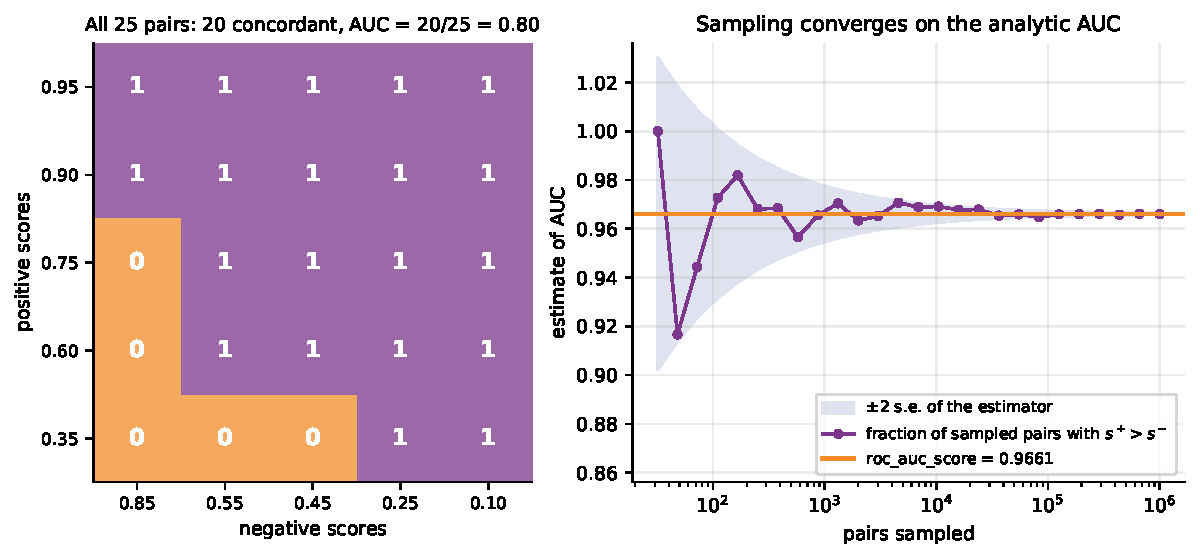
\includegraphics[width=\textwidth]{l19-auc-pairs.pdf}
\caption{Left: all $25$ positive--negative pairs from the ten hand rows; a $1$
marks a pair the model ordered correctly. Twenty of twenty-five, AUC $0.80$.
Right: the sampled estimate on \texttt{breast\_cancer} converging on the
analytic AUC, inside the $\pm 2$ standard-error band of a Bernoulli proportion.}
\label{fig:pairs}
\end{figure}

\subsection{What $0.5$, and less than $0.5$, mean}

Give a model no information at all and it lands on the diagonal:

\begin{lstlisting}
rng = np.random.default_rng(0)            # the one seed for this lecture
yr, sr = rng.integers(0, 2, 2000), rng.random(2000)
print(roc_auc_score(yr, sr))
\end{lstlisting}
\begin{codeout}
2000 coin-flip labels, 2000 uniform random scores
  roc_auc_score  0.5023
  accuracy at threshold 0.5  0.5090
  200 repetitions: mean 0.4994  sd 0.0136  min 0.4645  max 0.5342
  the diagonal is not a curve you draw, it is the answer you get
  when the score carries no information about the label.
\end{codeout}

Two hundred repetitions give a mean of $0.4994$ and a standard deviation of
$0.0136$; the extremes are $0.4645$ and $0.5342$. That spread is the useful part:
on $2000$ rows, an AUC of $0.53$ is \emph{not evidence of anything}.

An AUC below $0.5$ is a different animal.

\begin{lstlisting}
print(roc_auc_score(yb_te, sb), roc_auc_score(yb_te, -sb),
      roc_auc_score(1 - yb_te, sb))
\end{lstlisting}
\begin{codeout}
the fitted breast_cancer model              AUC 0.9661
the same model with its scores negated      AUC 0.0339
the same model with the labels swapped      AUC 0.0339
1 - AUC                                         0.0339
An AUC of 0.0339 is not a bad model. It is this model wired backwards:
flip the sign of the score and you get 0.9661 back.
\end{codeout}

\begin{keyidea}
$\mathrm{AUC}(-s) = 1 - \mathrm{AUC}(s)$, exactly, because negating the score
reverses every pairwise comparison. So $0.5$, not $0$, is the floor for a model
you are allowed to relabel. An AUC well below $0.5$ almost always means you have
passed the wrong column of \texttt{predict\_proba}, or defined the positive class
one way and scored it the other.
\end{keyidea}

\begin{figure}[htbp]
\centering
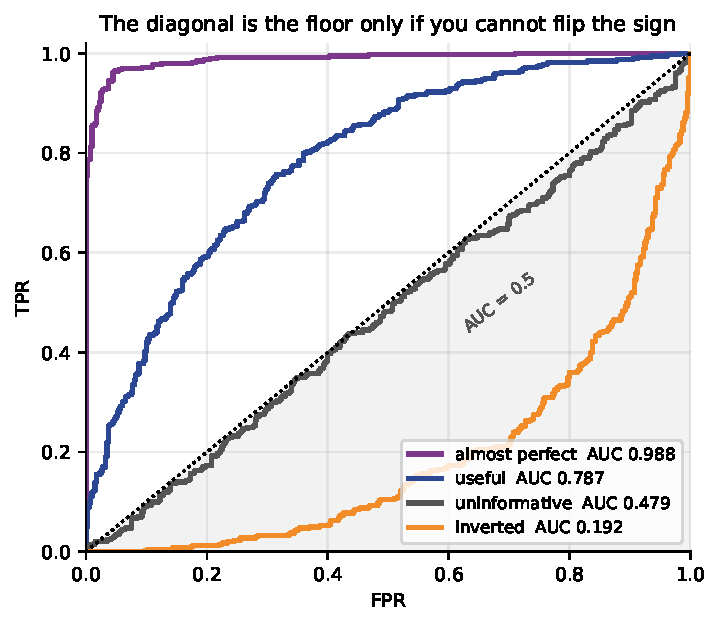
\includegraphics[width=0.62\textwidth]{l19-roc-families.pdf}
\caption{Four ROC curves on synthetic data of decreasing quality. The
``inverted'' curve at AUC $0.192$ becomes AUC $0.808$ the moment you flip the
sign of its score.}
\label{fig:families}
\end{figure}

\subsection{The two invariances}

\textbf{AUC does not depend on the threshold.} That is not a property to be
proved; it is a consequence of the construction. Look again at the sweep table
in Section~\ref{sec:rochand}: the threshold appears as a row label, not as an
input. The seven-row table of Section~\ref{sec:scores} makes the same point from
the other side --- accuracy moved from $0.7135$ to $0.9181$ across thresholds
while AUC stayed at $0.9661$ throughout.

\textbf{AUC does not depend on the class balance.} Keep every positive and throw
away negatives at random; $\TPR$ is computed within the positives and $\FPR$
within the negatives, so neither is systematically disturbed.

\begin{lstlisting}
for k in [5940, 2000, 500, 120, 60]:
    sel = np.concatenate([idx_pos, perm_of_negatives[:k]])
    print(k, yi_te[sel].mean(), roc_auc_score(yi_te[sel], si[sel]),
          average_precision_score(yi_te[sel], si[sel]))
\end{lstlisting}
\begin{codeout}
same model, same scores; only the negatives are subsampled
 negatives kept  prevalence   ROC AUC   avg precision
           5940      0.0100    0.9200       0.1702
           2000      0.0291    0.9197       0.3380
            500      0.1071    0.9172       0.6699
            120      0.3333    0.9243       0.8839
             60      0.5000    0.9158       0.9202
ROC AUC is invariant to class balance. Average precision is not:
  it rose from 0.1702 to 0.9202 -- a factor of 5.4 -- without the model
  changing at all.
\end{codeout}

ROC AUC stayed inside a band of $0.0085$, from $0.9158$ to $0.9243$, over a
fiftyfold change in prevalence --- sampling noise, and in no particular
direction. Average precision moved by a factor of $5.4$. That single table is the
whole of the next section.

% =========================================================================
\section{ROC against precision--recall}
\label{sec:rocpr}

\subsection{The case where ROC flatters}

Return to the $99\!:\!1$ problem of Section~\ref{sec:whynot}: $6000$ held-out
rows, $60$ of them positive, logistic regression.

\begin{lstlisting}
from sklearn.metrics import precision_recall_curve, average_precision_score
print("ROC AUC          ", roc_auc_score(yi_te, si))
print("average precision", average_precision_score(yi_te, si))
prec, rec, thr = precision_recall_curve(yi_te, si)
\end{lstlisting}
\begin{codeout}
the 99:1 problem, logistic regression, 6000 held-out rows
  prevalence            0.0100  (60 positives, 5940 negatives)
  ROC AUC               0.9200   (baseline 0.5000)
  average precision     0.1702   (baseline = prevalence = 0.0100)

  recall   precision   threshold    TP    FP
   0.10      0.2400      0.3634       6    19
   0.30      0.2647      0.2004      18    50
   0.50      0.1648      0.0719      30   152
   0.70      0.0955      0.0275      42   398
   0.90      0.0439      0.0069      54  1177
   1.00      0.0100      0.0000      60  5940

  ROC reads: at TPR 0.9000 the FPR is only 0.1946 -- encouraging.
  PR reads:  0.1946 x 5940 = 1156 false alarms for 54 true ones,
             precision 0.0446. One alert in 22 is real.
\end{codeout}

An AUC of $0.9200$ against a baseline of $0.5$ reads as a strong model. It
\emph{is} a strong model, in the precise sense that AUC measures: pick a random
positive and a random negative and it orders them correctly $92\%$ of the time.
That claim is true and it is not the claim the person paying for the system
cares about.

The precision--recall curve answers their question instead. To catch $90\%$ of
the positives you must accept $1156$ false alarms alongside $54$ real ones. The
$\FPR$ of $0.1946$ that looked small on the ROC axis is $19.46\%$ of $5940$
negatives, and $5940$ is a large number.

\begin{keyidea}
$\FPR = \FP/N$ divides by the number of negatives, which is huge when the
positives are rare, so a large absolute number of false alarms shows up as a
small $\FPR$. Precision divides by $\TP + \FP$ instead, and when $\FP$ swamps
$\TP$ it falls off a cliff. \textbf{Under heavy imbalance ROC is optimistic
because its denominator is generous.}
\end{keyidea}

\begin{figure}[htbp]
\centering
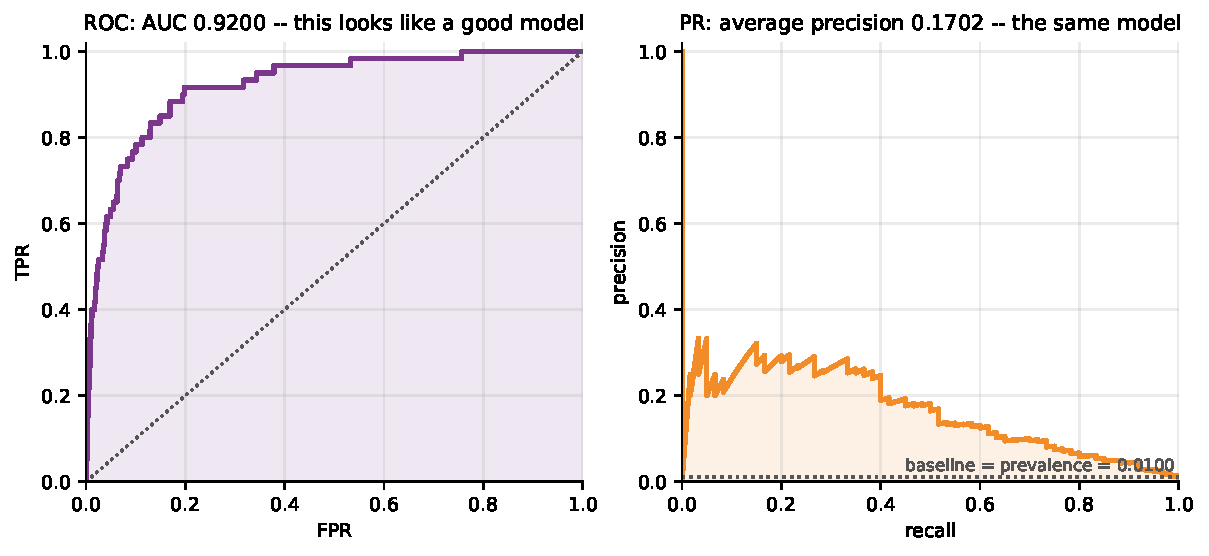
\includegraphics[width=\textwidth]{l19-roc-vs-pr.pdf}
\caption{The same model, the same scores, the same $6000$ rows. Left: ROC,
AUC $0.9200$. Right: precision--recall, average precision $0.1702$ against a
prevalence baseline of $0.0100$. Neither picture is wrong; they answer different
questions.}
\label{fig:rocpr}
\end{figure}

\subsection{Baselines, and how to read the two plots}

\begin{center}\small
\begin{tabular}{@{}llll@{}}
\toprule
 & axes & baseline of a useless model & depends on prevalence?\\
\midrule
ROC & $\TPR$ against $\FPR$ & the diagonal, AUC $= 0.5$ & no\\
PR  & precision against recall & the horizontal line at the prevalence & yes\\
\bottomrule
\end{tabular}
\end{center}

A PR curve has no fixed baseline, which is the first thing students get wrong
about it. On a balanced problem a useless model achieves precision $0.5$
everywhere; at $1\%$ prevalence it achieves $0.01$. So an average precision of
$0.17$ at $1\%$ prevalence is \emph{seventeen times} the baseline --- a real
achievement --- while an average precision of $0.17$ on a balanced problem would
be worse than guessing. Always quote the prevalence next to the average
precision.

\begin{figure}[htbp]
\centering
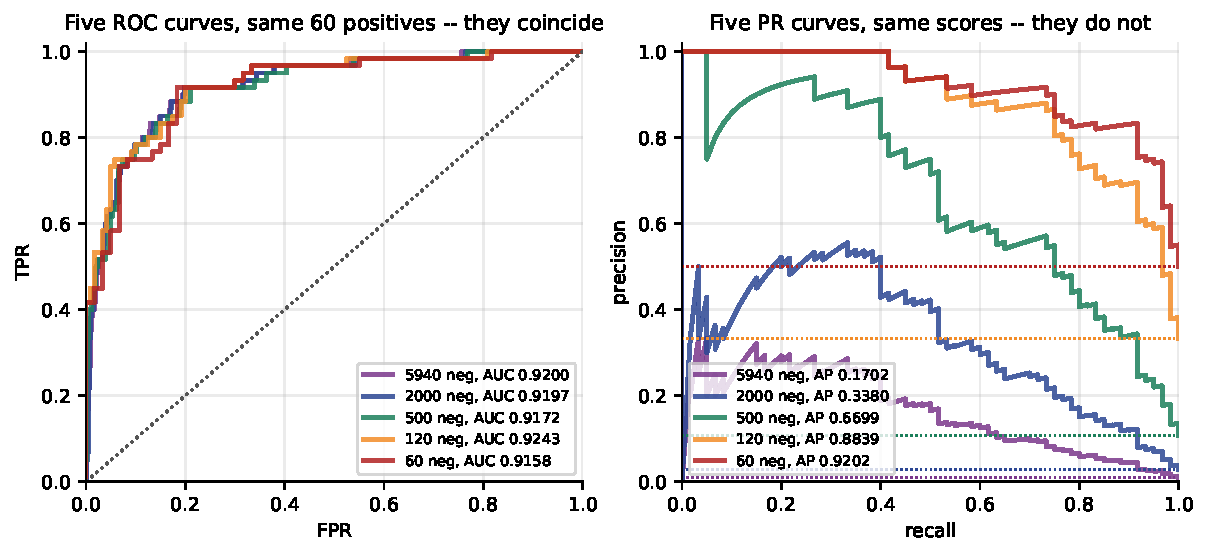
\includegraphics[width=\textwidth]{l19-balance-invariance.pdf}
\caption{Five evaluations of one fixed set of scores, differing only in how many
negatives were kept. Left: the ROC curves lie on top of each other. Right: the
PR curves fan out, and their dotted baselines move with them.}
\label{fig:balance}
\end{figure}

\subsection{Which to report}

\begin{itemize}[leftmargin=*]
  \item Report \textbf{ROC AUC} when the two classes are comparably common, when
    you want a summary that will not shift because next month's data has a
    different mix, or when the cost of a false positive and a false negative are
    of the same order.
  \item Report \textbf{average precision} (or the PR curve) when positives are
    rare and the consumer of the model is going to act on the alerts. Anything
    with a human in the loop --- fraud review, medical triage, moderation --- is
    in this category, because a human has finite capacity and precision is
    exactly the fraction of their time that is not wasted.
  \item \textbf{Report both.} They are two lines of code and they answer
    different questions. Saito and Rehmsmeier's 2015 paper is the standard
    citation for preferring PR under imbalance; it is in the references.
\end{itemize}

\begin{caution}
The invariance runs both ways, and the second direction is the dangerous one.
Because ROC AUC does not move with the class balance, an AUC measured on a
balanced sample of your data \emph{transfers} to the imbalanced population ---
which is convenient. Average precision does not transfer: if you undersample the
negatives for training and then evaluate on the undersampled set, your reported
average precision will be several times what you will see in production. The
final evaluation goes on data with the production prevalence.
\end{caution}

% =========================================================================
\section{Choosing the threshold is a business decision}
\label{sec:threshold}

\subsection{$0.5$ is an assumption, not a default}

\texttt{predict} thresholds at $0.5$. That choice is optimal under exactly one
condition: a false positive and a false negative cost the same. Nobody ever
checks whether that is true, and it almost never is. A missed tumour and an
unnecessary follow-up scan are not the same event.

Three ways to pick a threshold on purpose.

\subsection{Youden's $J$}

Youden's statistic is $J = \TPR - \FPR = \text{sensitivity} + \text{specificity}
- 1$. Maximising it picks the point on the ROC curve furthest above the diagonal,
measured vertically.

\begin{worked}[Youden on the ten hand rows]
\begin{center}\small
\begin{tabular}{@{}rrrr@{}}
\toprule
threshold & $\FPR$ & $\TPR$ & $J = \TPR - \FPR$\\
\midrule
$\infty$ & $0.0$ & $0.0$ & $0.0$\\
$0.95$ & $0.0$ & $0.2$ & $0.2$\\
$0.90$ & $0.0$ & $0.4$ & $0.4$\\
$0.85$ & $0.2$ & $0.4$ & $0.2$\\
$0.75$ & $0.2$ & $0.6$ & $0.4$\\
$\mathbf{0.60}$ & $\mathbf{0.2}$ & $\mathbf{0.8}$ & $\mathbf{0.6}$\\
$0.55$ & $0.4$ & $0.8$ & $0.4$\\
$0.45$ & $0.6$ & $0.8$ & $0.2$\\
$0.35$ & $0.6$ & $1.0$ & $0.4$\\
$0.25$ & $0.8$ & $1.0$ & $0.2$\\
$0.10$ & $1.0$ & $1.0$ & $0.0$\\
\bottomrule
\end{tabular}
\end{center}
The maximum is $J = 0.6$ at threshold $0.60$, giving $(\FPR, \TPR) = (0.2, 0.8)$.
\end{worked}

On the three-feature \texttt{breast\_cancer} model with \emph{malignant} as the
positive class:

\begin{codeout}
the same rule on breast_cancer, malignant as the positive class:
  Youden threshold 0.3612   J 0.8160   FPR 0.1215   TPR 0.9375
  at t = 0.5000: recall 0.8594  precision 0.8871  accuracy 0.9064
  at Youden    : recall 0.9375  precision 0.8219  accuracy 0.9006
\end{codeout}

Youden buys eight points of recall on the class you must not miss, for six points
of precision and half a point of accuracy. Whether that is a good trade is not a
statistical question.

\begin{caution}
Youden's $J$ weights a unit of sensitivity and a unit of specificity equally, so
it is the equal-cost answer wearing different clothes. It is a reasonable
\emph{default} when nobody will tell you the costs, and it is the wrong answer
the moment somebody does.
\end{caution}

\subsection{The cost-weighted choice}

Assign a cost $C_{\FN}$ to a miss and $C_{\FP}$ to a false alarm and choose the
threshold that minimises the expected total,
\begin{equation}
\text{cost}(t) \;=\; C_{\FN} \cdot \FN(t) \;+\; C_{\FP} \cdot \FP(t).
\label{eq:cost}
\end{equation}
Only the \emph{ratio} matters, so fix $C_{\FP} = 1$ and vary $C_{\FN}$.

\begin{worked}[The costed sweep, ten rows]
\begin{center}\small
\begin{tabular}{@{}rrrrrrr@{}}
\toprule
threshold & $\TP$ & $\FP$ & $\FN$ & $\TN$ & cost at $1\!:\!1$ & cost at $10\!:\!1$\\
\midrule
$0.95$ & 1 & 0 & 4 & 5 & $4$ & $40$\\
$0.90$ & 2 & 0 & 3 & 5 & $3$ & $30$\\
$0.85$ & 2 & 1 & 3 & 4 & $4$ & $31$\\
$0.75$ & 3 & 1 & 2 & 4 & $3$ & $21$\\
$\mathbf{0.60}$ & 4 & 1 & 1 & 4 & $\mathbf{2}$ & $11$\\
$0.55$ & 4 & 2 & 1 & 3 & $3$ & $12$\\
$0.45$ & 4 & 3 & 1 & 2 & $4$ & $13$\\
$\mathbf{0.35}$ & 5 & 3 & 0 & 2 & $3$ & $\mathbf{3}$\\
$0.25$ & 5 & 4 & 0 & 1 & $4$ & $4$\\
$0.10$ & 5 & 5 & 0 & 0 & $5$ & $5$\\
\bottomrule
\end{tabular}
\end{center}
At $1\!:\!1$ the cheapest threshold is $0.60$, costing $2$: that is
$(\TPR, \FPR) = (0.80, 0.20)$, and it is Youden's answer, as it must be on a
balanced set with equal costs.

At $10\!:\!1$ the cheapest threshold is $0.35$, costing $3$: that is
$(\TPR, \FPR) = (1.00, 0.60)$. \textbf{Making a miss ten times as expensive moved
the threshold from $0.60$ to $0.35$, took recall from $0.80$ to $1.00$, and
tripled the false alarm rate.} Read down the $10\!:\!1$ column and watch the
minimum walk left as the price of a miss rises.
\end{worked}

On \texttt{breast\_cancer}, malignant positive, over a grid of cost ratios:

\begin{lstlisting}
grid = np.unique(sm)                     # sm = 1 - sb, malignant score
for ratio in [1, 2, 5, 10, 20, 50]:
    costs = [ratio * FN(t) + FP(t) for t in grid]
    t = grid[int(np.argmin(costs))]
\end{lstlisting}
\begin{codeout}
the same costing on breast_cancer; malignant is now the positive
malignant 64   benign 107   ROC AUC 0.9661
C_FN:C_FP   threshold   cost   FN   FP   recall  precision
    1:1       0.6855     14   13    1   0.7969    0.9808
    2:1       0.3612     21    4   13   0.9375    0.8219
    5:1       0.3612     33    4   13   0.9375    0.8219
   10:1       0.0670     42    0   42   1.0000    0.6038
   20:1       0.0670     42    0   42   1.0000    0.6038
   50:1       0.0670     42    0   42   1.0000    0.6038
Raising the price of a miss from 1 to 10 moved the threshold from 0.6855 to 0.0670,
recall from 0.7969 to 1.0000 and precision from 0.6038 ... 0.9808 to 0.6038.
Nothing about the model changed. Only the price list.
\end{codeout}

\begin{keyidea}
At $1\!:\!1$ this model misses $13$ of $64$ malignant cases and raises one false
alarm. At $10\!:\!1$ it misses none and raises $42$. \textbf{Same model, same
scores, same day --- a completely different clinical instrument.} Report the
threshold with the model, always, and say where it came from.
\end{keyidea}

Two honest observations from that table. The cost curve is a step function with
finitely many breakpoints, so a \emph{range} of cost ratios shares an optimum:
here $2\!:\!1$ and $5\!:\!1$ both pick $0.3612$, and everything from $10\!:\!1$
upwards picks $0.0670$. And once the threshold is low enough that $\FN = 0$,
raising the price of a miss further changes nothing --- you cannot buy fewer than
zero misses.

\begin{figure}[htbp]
\centering
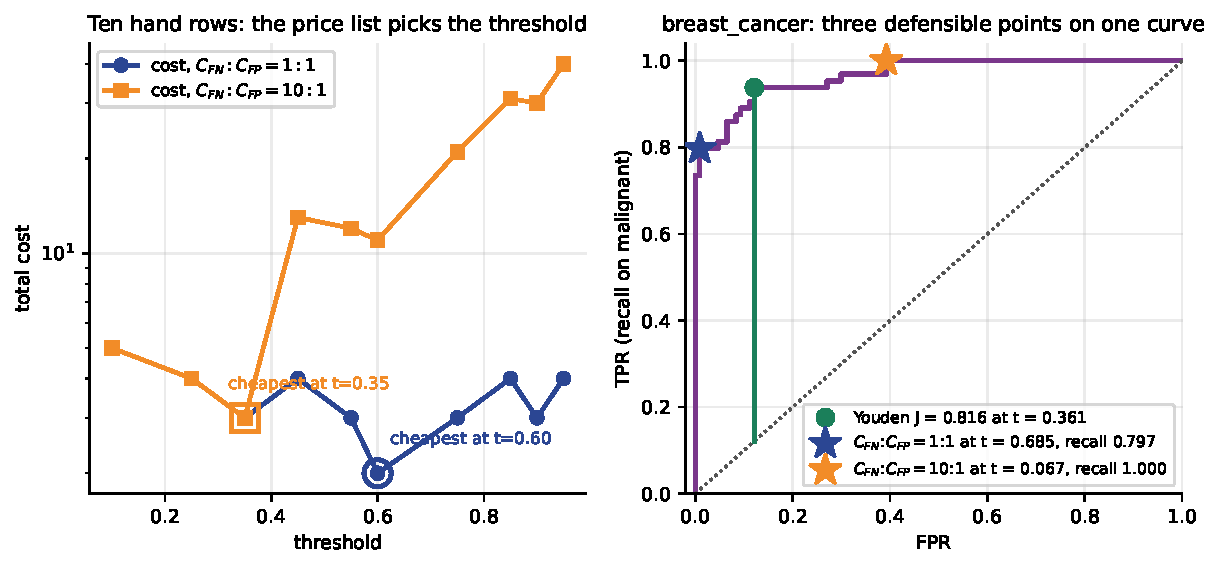
\includegraphics[width=\textwidth]{l19-cost-threshold.pdf}
\caption{Left: total cost against threshold on the ten hand rows, at
$1\!:\!1$ and $10\!:\!1$; the minima are at $0.60$ and $0.35$. Right: three
defensible operating points on one \texttt{breast\_cancer} ROC curve. The curve
is the model; the points are decisions.}
\label{fig:cost}
\end{figure}

\subsection{Where the threshold is chosen}

\begin{caution}[The threshold is a parameter, and parameters leak]
Choosing the threshold that maximises $J$, or minimises cost, \textbf{on the test
set} is fitting to the test set. It is a small leak compared with the feature
selection of Lecture~6, but it is the same kind of error. Choose the threshold on
a validation split or inside the cross-validation folds; report on the test set
once, at the threshold you already chose. scikit-learn's
\texttt{TunedThresholdClassifierCV} does exactly this and can be dropped into a
\texttt{Pipeline}.
\end{caution}

% =========================================================================
\section{More than two classes}
\label{sec:multi}

\subsection{The $k \times k$ confusion matrix}

With $k$ classes the confusion matrix is $k \times k$: entry $(i, j)$ is the
number of rows whose true class is $i$ and whose predicted class is $j$. The
diagonal is correct, everything else is a specific kind of mistake, and the
off-diagonal pattern is often more informative than any summary --- a model that
confuses $3$ with $8$ has a different problem from one that confuses $3$ with
$5$.

Precision, recall and $F_1$ are defined per class, one-vs-rest: for class $i$,
$\TP_i$ is the diagonal entry, $\FP_i$ is the rest of column $i$, $\FN_i$ is the
rest of row $i$. Then the question is how to average $k$ numbers into one, and
there are three answers that routinely disagree.

\subsection{Micro, macro and weighted, by hand}

\begin{worked}[One hundred rows, three classes]
\begin{center}\small
\begin{tabular}{@{}lrrrr@{}}
\toprule
 & pred A & pred B & pred C & row total\\
\midrule
actual A & $54$ & $4$ & $2$ & $60$\\
actual B & $6$ & $21$ & $3$ & $30$\\
actual C & $4$ & $2$ & $4$ & $10$\\
\midrule
column total & $64$ & $27$ & $9$ & $100$\\
\bottomrule
\end{tabular}
\end{center}

Accuracy is the diagonal over the total: $(54 + 21 + 4)/100 = 0.79$.

Per class, with $\TP_i$ on the diagonal, $\FP_i = (\text{column sum}) - \TP_i$
and $\FN_i = (\text{row sum}) - \TP_i$:
\begin{center}\small
\begin{tabular}{@{}lrrrrrrr@{}}
\toprule
class & $\TP$ & $\FP$ & $\FN$ & support & precision & recall & $F_1$\\
\midrule
A & $54$ & $10$ & $6$ & $60$ & $54/64 = 0.843750$ & $54/60 = 0.900000$ & $0.870968$\\
B & $21$ & $6$  & $9$ & $30$ & $21/27 = 0.777778$ & $21/30 = 0.700000$ & $0.736842$\\
C & $4$  & $5$  & $6$ & $10$ & $4/9  = 0.444444$ & $4/10 = 0.400000$ & $0.421053$\\
\bottomrule
\end{tabular}
\end{center}

Now the three averages.

\textbf{Micro} pools the counts before dividing:
$\sum \TP = 79$, $\sum \FP = 21$, $\sum \FN = 21$, so micro precision
$= 79/100 = 0.79$, micro recall $= 79/100 = 0.79$, micro $F_1 = 0.79$. In
single-label multiclass all three equal accuracy --- always, because every row
contributes exactly one $\TP$ or one $\FP$ and one $\FN$.

\textbf{Macro} is the unweighted mean of the per-class numbers:
\begin{align*}
\text{macro precision} &= \tfrac{1}{3}(0.843750 + 0.777778 + 0.444444) = 0.688657\\
\text{macro recall}    &= \tfrac{1}{3}(0.900000 + 0.700000 + 0.400000) = 0.666667\\
\text{macro } F_1      &= \tfrac{1}{3}(0.870968 + 0.736842 + 0.421053) = 0.676287
\end{align*}

\textbf{Weighted} uses the supports $60, 30, 10$ as weights:
\begin{align*}
\text{weighted precision} &= \tfrac{60(0.843750) + 30(0.777778) + 10(0.444444)}{100} = 0.784028\\
\text{weighted recall}    &= \tfrac{60(0.9) + 30(0.7) + 10(0.4)}{100} = \tfrac{54 + 21 + 4}{100} = 0.790000\\
\text{weighted } F_1      &= \tfrac{60(0.870968) + 30(0.736842) + 10(0.421053)}{100} = 0.785739
\end{align*}

Two facts fall out. Weighted recall equals accuracy --- it always does, because
$\sum_i n_i (\TP_i / n_i) = \sum_i \TP_i$. And macro $F_1$ is $0.1095$
\emph{below} weighted $F_1$, because class C is a tenth of the rows and a third
of the macro vote, and the model is bad at it.
\end{worked}

\begin{lstlisting}
print(classification_report(y_true3, y_pred3, digits=6,
                            target_names=["A", "B", "C"]))
\end{lstlisting}
\begin{codeout}
              precision    recall  f1-score   support

           A   0.843750  0.900000  0.870968        60
           B   0.777778  0.700000  0.736842        30
           C   0.444444  0.400000  0.421053        10

    accuracy                       0.790000       100
   macro avg   0.688657  0.666667  0.676287       100
weighted avg   0.784028  0.790000  0.785739       100
\end{codeout}

Every hand figure, to six decimal places.

\begin{keyidea}
\textbf{Micro} asks ``how often is the model right?'' and equals accuracy.
\textbf{Macro} asks ``how well does it do on a typical \emph{class}?'' and gives
the rarest class the same vote as the commonest. \textbf{Weighted} asks ``how
well does it do on a typical \emph{row}?''. Choose by deciding who you are
answerable to: a per-class regulator wants macro, a throughput target wants
micro.
\end{keyidea}

\subsection{The same on real data}

Take \texttt{load\_digits} and make two of its classes rare on purpose: keep only
$20$ examples each of the digits $3$ and $8$.

\begin{codeout}
imbalanced digits: 1480 rows, class counts [178 182 177  20 181 182 181 179  20 180]
accuracy 0.9662
  micro     precision 0.9662  recall 0.9662  F1 0.9662
  macro     precision 0.9730  recall 0.9131  F1 0.9339
  weighted  precision 0.9669  recall 0.9662  F1 0.9652
per-class recall: [1.     0.9818 0.9811 0.8333 0.963  0.9273 0.9815 0.9815 0.5    0.9815]
classes 3 and 8 have 6 test rows each and recall 0.8333 and 0.5000.
micro hides them completely; macro is the only average that shows them.
\end{codeout}

Micro and weighted both read $0.97$. Macro reads $0.93$ and macro \emph{recall}
reads $0.9131$ --- because the model finds half of the eights. If the
eights are the cases you care about, only the macro row and the per-class array
told you anything.

\subsection{One-vs-rest ROC}

ROC needs a positive class, so multiclass ROC means $k$ curves: for each class,
score that class against all the others. \texttt{roc\_auc\_score} does this with
\texttt{multi\_class="ovr"}, and averages with \texttt{average="macro"} or
\texttt{"weighted"}. There is also \texttt{"ovo"}, which averages over all
$\binom{k}{2}$ pairwise AUCs and is the more natural choice when the class sizes
are wildly different.

A three-class problem at $80 / 15 / 5$:

\begin{lstlisting}
P3 = model.predict_proba(X3_te)
for c in range(3):
    print(c, roc_auc_score((y3_te == c).astype(int), P3[:, c]))
print(roc_auc_score(y3_te, P3, multi_class="ovr", average="macro"))
print(roc_auc_score(y3_te, P3, multi_class="ovr", average="weighted"))
\end{lstlisting}
\begin{codeout}
three classes, [709 140  51] in the test set
accuracy 0.8600

class  support   one-vs-rest AUC   recall      F1
  0        709          0.8920     0.9633  0.9236
  1        140          0.9090     0.6500  0.6766
  2         51          0.7793     0.0000  0.0000

macro    OvR AUC 0.8601   F1 0.5334
weighted OvR AUC 0.8883   F1 0.8328
micro                       F1 0.8600 (= accuracy 0.8600)
macro OvO AUC 0.8151

macro F1 0.5334 against weighted F1 0.8328: a gap of 0.2994.
Report the one that matches who you will disappoint.
\end{codeout}

\begin{caution}[The most instructive row in these notes]
Class $2$ has \textbf{recall $0.0000$ and $F_1$ $0.0000$} --- the model never
predicts it, not once --- and yet its one-vs-rest \textbf{AUC is $0.7793$}.
There is real information in the scores for class $2$; \texttt{argmax} simply
never lets it win, because class $0$ is sixteen times as common and the prior
buries it. AUC sees the ranking; $F_1$ sees only the decision. If you had
reported weighted $F_1 = 0.8328$ and stopped, you would have shipped a model
that cannot detect one of its three classes at all.
\end{caution}

\begin{figure}[htbp]
\centering
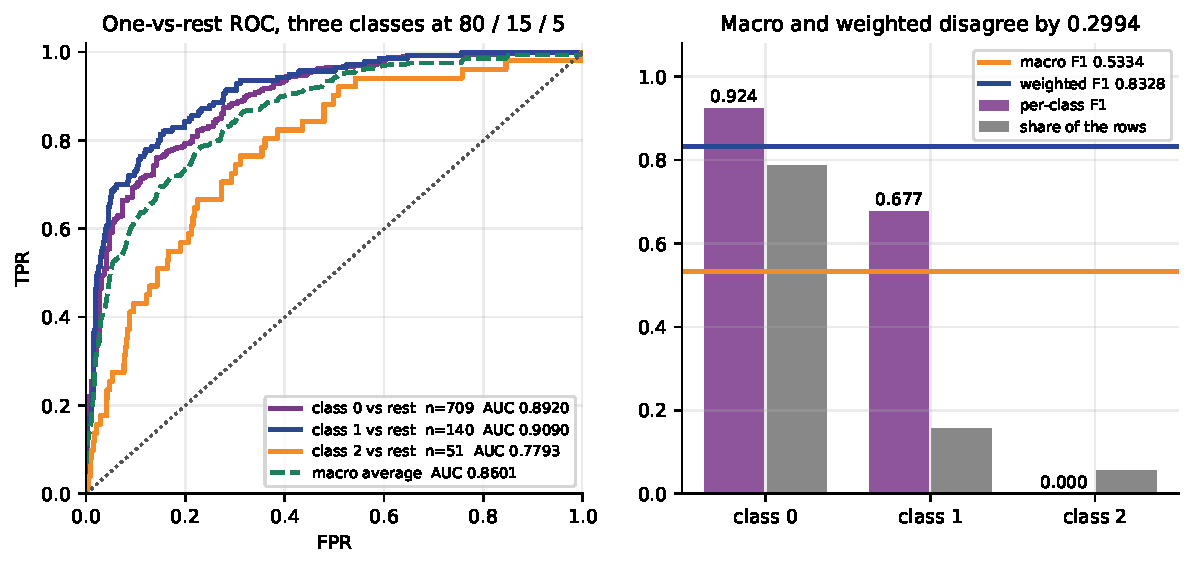
\includegraphics[width=\textwidth]{l19-multiclass-ovr.pdf}
\caption{Left: three one-vs-rest ROC curves and their macro average, on a
$80/15/5$ problem. Right: the per-class $F_1$ against the class share, with the
macro and weighted averages as horizontal lines. They differ by $0.2994$.}
\label{fig:multiclass}
\end{figure}

% =========================================================================
\section{Model selection, done properly}
\label{sec:selection}

\subsection{Cross-validated AUC, with error bars}

Now the question the unit has been building to: given the classifiers of
Lectures~13 to~18, which one? The wrong way is a single train/test split and a
single accuracy. The right way is a repeated, stratified cross-validation with
a metric chosen in advance and an honest report of the spread.

\begin{lstlisting}
from sklearn.model_selection import RepeatedStratifiedKFold, cross_val_score
models = {
  "KNN (k=5)":     make_pipeline(StandardScaler(), KNeighborsClassifier(5)),
  "Decision tree": DecisionTreeClassifier(random_state=0),
  "Gaussian NB":   GaussianNB(),
  "Random forest": RandomForestClassifier(n_estimators=300, random_state=0),
  "SVM (RBF)":     make_pipeline(StandardScaler(),
                                 SVC(probability=True, random_state=0)),
  "MLP (100)":     make_pipeline(StandardScaler(),
                                 MLPClassifier(hidden_layer_sizes=(100,),
                                               max_iter=2000, random_state=0)),
  "Logistic reg.": make_pipeline(StandardScaler(),
                                 LogisticRegression(max_iter=5000)),
}
cv = RepeatedStratifiedKFold(n_splits=5, n_repeats=4, random_state=0)
# 20 folds: the spread between them is the point, and seed 0 makes it repeat
res = {n: cross_val_score(m, Xb, yb, cv=cv, scoring="roc_auc")
       for n, m in models.items()}
\end{lstlisting}
\begin{codeout}
breast_cancer, all 30 features, 5-fold x 4 repeats = 20 folds
model             mean AUC     sd   2 s.e.    worst    best
SVM (RBF)         0.9950  0.0058  0.0026   0.9771  1.0000
Logistic reg.     0.9948  0.0056  0.0025   0.9803  1.0000
MLP (100)         0.9944  0.0060  0.0027   0.9800  1.0000
Random forest     0.9905  0.0090  0.0040   0.9705  1.0000
Gaussian NB       0.9882  0.0069  0.0031   0.9705  0.9993
KNN (k=5)         0.9849  0.0107  0.0048   0.9633  1.0000
Decision tree     0.9227  0.0205  0.0092   0.8809  0.9554
\end{codeout}

Three notes on the machinery. \texttt{RepeatedStratifiedKFold} gives twenty
estimates rather than five, which is what makes the standard error worth
quoting. Every scaler sits inside a \texttt{Pipeline}, so it is refitted in each
fold --- Lecture~6's rule. And \texttt{scoring="roc\_auc"} was chosen before the
run, not after looking at the results.

\subsection{A difference smaller than the spread is not a difference}

The table above is easy to misread as a ranking. Look at the numbers instead.

\begin{codeout}
best   SVM (RBF)        0.9950
second Logistic reg.    0.9948
gap 0.0003;  fold-to-fold sd of the gap 0.0022
paired t = 0.598, p = 0.5569 over 20 folds
SVM (RBF) beat Logistic reg. on 7 of the 20 folds
\end{codeout}

The SVM's lead is $0.0003$. The fold-to-fold standard deviation of that lead is
$0.0022$, seven times larger, and the SVM actually \emph{lost} thirteen of the
twenty folds while winning on the mean. A paired $t$-test gives $p = 0.5569$.

\begin{keyidea}
$0.9950$ against $0.9948$ is not a result. The fold-to-fold spread is
$0.0058$; four of the seven models sit inside one such spread of the leader.
\textbf{When the gap is smaller than the noise, choose on something else:}
training time, interpretability, how it behaves on the tail of the data, whether
you can explain it to a clinician.
\end{keyidea}

\subsection{The ranking flips between folds}

\begin{codeout}
fold-by-fold, the top four models, first eight folds
fold  SVM (RBF)      Logistic reg.  MLP (100)      Random forest  winner
  0   0.9869         0.9846         0.9840         0.9813         SVM (RBF)
  1   0.9987         0.9990         0.9954         0.9990         Logistic reg.
  2   0.9967         0.9980         0.9974         0.9866         Logistic reg.
  3   1.0000         1.0000         1.0000         0.9964         SVM (RBF)
  4   0.9963         0.9956         0.9946         0.9980         Random forest
  5   0.9925         0.9905         0.9889         0.9880         SVM (RBF)
  6   0.9977         0.9987         0.9984         0.9838         Logistic reg.
  7   0.9983         0.9950         0.9997         0.9960         MLP (100)
\end{codeout}

Four different winners in eight folds. Over all twenty:

\begin{codeout}
how often does the fold-level winner change?
  Logistic reg.    won  7 of 20 folds
  SVM (RBF)        won  4 of 20 folds
  MLP (100)        won  4 of 20 folds
  Random forest    won  2 of 20 folds
  KNN (k=5)        won  2 of 20 folds
  Gaussian NB      won  1 of 20 folds

fold-to-fold sd of the leader: 0.0058
models within one sd of the leader: Logistic reg., MLP (100), Random forest, SVM (RBF)
A gap smaller than the fold-to-fold spread is not a difference.
\end{codeout}

Six of the seven models won at least one fold. Had you run a single $80/20$
split you would have crowned one of them, and which one would have been decided
by \texttt{random\_state}.

\begin{figure}[htbp]
\centering
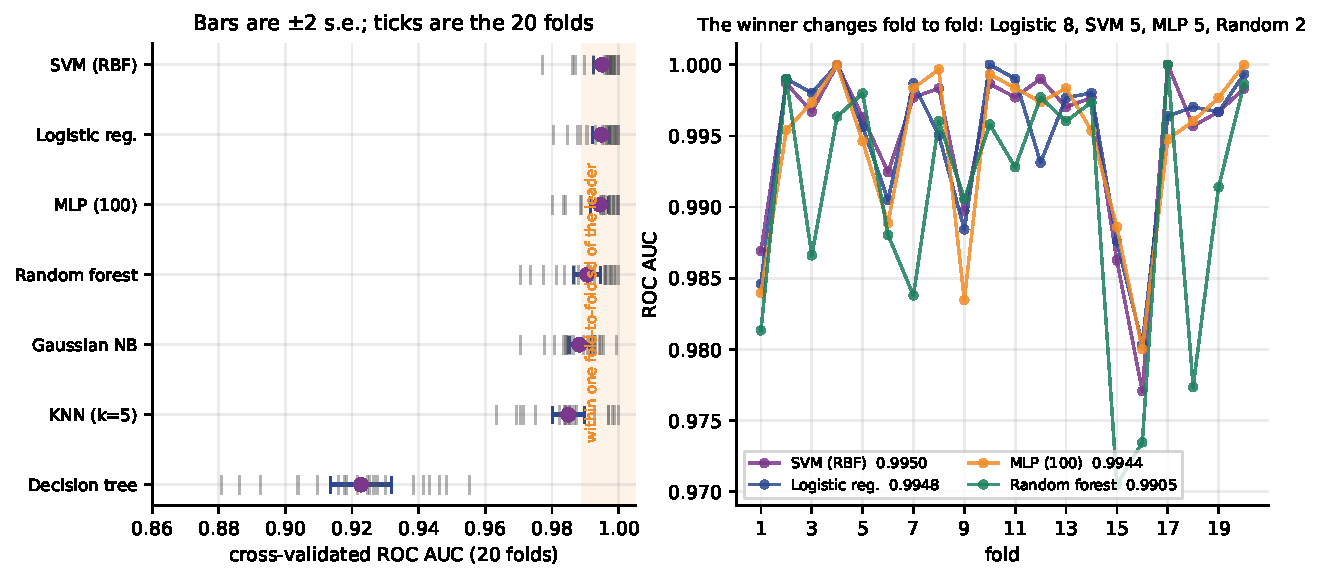
\includegraphics[width=\textwidth]{l19-model-selection.pdf}
\caption{Left: mean cross-validated AUC with $\pm 2$ standard-error bars; the
grey ticks are the twenty individual folds and the shaded band is one
fold-to-fold standard deviation of the leader. Right: the top four models fold
by fold. The lines cross constantly.}
\label{fig:selection}
\end{figure}

\subsection{The metric decides the ranking}

One more warning, and it closes the loop with Section~\ref{sec:whynot}. Score
those same seven models on the same folds by accuracy as well as AUC:

\begin{codeout}
the same seven models scored by accuracy and by AUC, same folds
model             accuracy     AUC    acc rank   AUC rank
SVM (RBF)         0.9771    0.9957       3          1
Logistic reg.     0.9789    0.9955       1          2
MLP (100)         0.9789    0.9943       2          3
Random forest     0.9578    0.9923       5          4
Gaussian NB       0.9385    0.9885       6          5
KNN (k=5)         0.9649    0.9806       4          6
Decision tree     0.9262    0.9210       7          7
models whose rank differs between the two metrics: 6 of 7
Pick the metric before you pick the model, and say why.
\end{codeout}

Six of the seven models change rank. $k$-NN is fourth by accuracy and sixth by
AUC; the random forest is fifth by accuracy and fourth by AUC. There is no
metric-free notion of ``the best model''.

\subsection{A checklist for the comparison you will write in A2}

\begin{enumerate}[leftmargin=*]
  \item State the positive class and the prevalence.
  \item State the metric \emph{before} you run anything, and say why that metric.
  \item Put every preprocessing step inside a \texttt{Pipeline}.
  \item Use repeated stratified cross-validation, not one split.
  \item Report mean, standard deviation and the number of folds --- never a mean
    alone.
  \item Include a baseline: \texttt{DummyClassifier}, and a single simple model.
  \item Plot the ROC curves together, and the PR curves too if positives are
    rare.
  \item Choose the threshold from a stated cost or constraint, on validation
    data.
  \item Say plainly when two models are indistinguishable, and give the
    non-statistical reason you picked one.
\end{enumerate}

% =========================================================================
\section{Summary}

\begin{enumerate}[leftmargin=*]
  \item Accuracy is a weighted summary and the weights are the class
    frequencies. At $1\%$ prevalence a constant predictor scored $0.9900$ and a
    useful logistic regression scored $0.9897$ --- \textbf{accuracy ranked them
    backwards} while AUC ranked them $0.5000$ against $0.9200$.
  \item The confusion matrix has four numbers and every metric in the lecture is
    a ratio of two of them. On twenty patients with $\TP = 6, \FP = 2,
    \FN = 4, \TN = 8$: accuracy $0.7000$, precision $0.7500$, recall $0.6000$,
    specificity $0.8000$, $\FPR = 0.2000$, $F_1 = 0.6667$. \texttt{sklearn}
    reproduces all six; note that \texttt{confusion\_matrix} is the transpose of
    the textbook layout.
  \item A classifier outputs a score; \texttt{predict} silently thresholds it.
    One fixed set of scores gave accuracies from $0.7135$ to $0.9181$ across
    seven thresholds, with AUC fixed at $0.9661$ throughout.
  \item An ROC curve is a sorted list and some bookkeeping: step up $1/P$ for a
    positive, right $1/N$ for a negative. The eleven-point hand sweep of ten
    rows matched \texttt{roc\_curve(drop\_intermediate=False)} exactly.
  \item AUC two ways, same answer. Trapezoids: $0.08 + 0.16 + 0.16 + 0.20 +
    0.20 = \mathbf{0.80}$. Concordant pairs: $\mathbf{20/25 = 0.80}$. It is the
    probability a random positive outranks a random negative, and it is the
    Mann--Whitney $U$ rescaled. Sampling ten million pairs on
    \texttt{breast\_cancer} converged to $0.966230$ against an analytic
    $0.966121$; counting all $6848$ pairs matched to $0.00\mathrm{e}{+}00$.
  \item AUC $0.5$ is chance ($200$ coin-flip repetitions: mean $0.4994$, sd
    $0.0136$). AUC below $0.5$ is an inverted classifier: $0.9661$ becomes
    $0.0339$ when you negate the score, and $\mathrm{AUC}(-s) = 1 -
    \mathrm{AUC}(s)$ exactly.
  \item AUC is invariant to the threshold by construction, and to the class
    balance by measurement: over a fiftyfold change in prevalence it moved
    inside a band of $0.0085$ while average precision moved
    $0.1702 \to 0.9202$.
  \item \textbf{Under heavy imbalance ROC flatters.} At $1\%$ prevalence,
    ROC AUC $0.9200$, average precision $0.1702$; at $90\%$ recall that is
    $1156$ false alarms for $54$ true ones and one alert in twenty-two is real.
    The PR baseline is the prevalence, not $0.5$.
  \item The threshold is a business decision. On the ten hand rows, $1\!:\!1$
    costs pick $0.60$ (recall $0.80$) and $10\!:\!1$ costs pick $0.35$ (recall
    $1.00$). On \texttt{breast\_cancer}, going from $1\!:\!1$ to $10\!:\!1$ moved
    the threshold $0.6855 \to 0.0670$, misses $13 \to 0$, false alarms $1 \to 42$.
    Youden's $J$ is the equal-cost answer in disguise.
  \item Multiclass: micro always equals accuracy; weighted recall always equals
    accuracy; macro gives the rarest class a full vote. On the hundred-row hand
    example macro $F_1 = 0.676287$ against weighted $0.785739$. On a $80/15/5$
    problem the gap was $0.2994$ --- and the class with $F_1 = 0.0000$ had a
    one-vs-rest AUC of $0.7793$.
  \item Model selection: over $20$ folds the best two of seven classifiers
    differed by $0.0003$ with a fold-to-fold spread of $0.0058$, $p = 0.5569$,
    and the leader lost $13$ of $20$ folds. Six of seven models changed rank when
    the metric changed from AUC to accuracy. \textbf{A difference smaller than
    the fold-to-fold spread is not a difference.}
\end{enumerate}

% =========================================================================
\section{Practice questions}

Attempt these before reading Section~\ref{sec:solutions}. Questions 1, 2, 3, 5
and 7 are pure hand arithmetic and are the ones most likely to appear on a paper.

\begin{enumerate}[leftmargin=*]
  \item\label{q:cm} A spam filter is run on $200$ messages, of which $50$ are
    spam. It flags $60$ messages, and $40$ of those flagged really are spam.
    (a) Write out the full confusion matrix with spam as the positive class.
    (b) Compute accuracy, precision, recall, specificity, $\FPR$ and $F_1$.
    (c) Compute $F_2$ from Equation~\eqref{eq:fbeta}, and say in one sentence
    when you would prefer it to $F_1$ for this problem.

  \item\label{q:imb} A rare-disease screen has prevalence $0.2\%$ in a
    population of $50{,}000$. (a) What accuracy does a model that always answers
    ``healthy'' achieve? (b) A real model achieves recall $0.80$ and
    $\FPR = 0.05$. Fill in its confusion matrix. (c) What is its accuracy, and
    what is its precision? (d) Which of the two models would you deploy, and
    which number in your answer makes the case?

  \item\label{q:roc} Eight scored examples, four positive and four negative:
    \begin{center}\small
    \begin{tabular}{@{}lrrrrrrrr@{}}
    \toprule
    label & POS & neg & POS & POS & neg & POS & neg & neg\\
    score & $0.92$ & $0.88$ & $0.80$ & $0.66$ & $0.55$ & $0.40$ & $0.31$ & $0.15$\\
    \bottomrule
    \end{tabular}
    \end{center}
    (a) Sweep the threshold and tabulate $(\FPR, \TPR)$ at every step, starting
    from $(0,0)$. (b) Sketch the staircase. (c) Compute the AUC by trapezoids.
    (d) Compute it again by counting concordant pairs, and confirm the two agree.
    (e) Which threshold maximises Youden's $J$?

  \item\label{q:invert} A colleague reports an AUC of $0.23$ on a binary problem
    and concludes that the model is useless. (a) What is the model's AUC if you
    negate its scores? (b) Give two concrete coding mistakes that produce an AUC
    below $0.5$. (c) Why is $0.5$, and not $0$, the right floor to compare
    against?

  \item\label{q:cost} Using the eight examples of question~\ref{q:roc}: a false
    negative costs $8$ units and a false positive costs $1$. (a) Tabulate the
    total cost at every threshold. (b) Which threshold is cheapest? (c) Which
    threshold would you choose if the costs were equal? (d) Explain in one
    sentence why the cost-optimal threshold does not change continuously as you
    raise $C_{\FN}$.

  \item\label{q:pr} A fraud model is evaluated on $100{,}000$ transactions of
    which $500$ are fraudulent. At its chosen threshold it catches $400$ frauds
    and raises $9600$ false alarms. (a) Compute recall, $\FPR$ and precision.
    (b) The team reports ``$\FPR$ is under $10\%$''. Why is that a misleading
    way to describe the system? (c) The reviewers can examine $1000$ cases a
    day. What does that constraint say about which curve should be plotted, and
    about the threshold?

  \item\label{q:multi} A three-class model produces the confusion matrix
    (rows actual, columns predicted)
    $\begin{pmatrix} 80 & 10 & 10\\ 5 & 30 & 5\\ 5 & 5 & 10 \end{pmatrix}$.
    (a) Compute per-class precision, recall and $F_1$. (b) Compute micro, macro
    and weighted $F_1$. (c) Verify that weighted recall equals accuracy.
    (d) Which average would you report to a regulator who cares about the rarest
    class, and why?

  \item\label{q:select} Two classifiers are compared with $10$-fold
    cross-validated AUC. Model X: mean $0.8710$, sd $0.0290$. Model Y: mean
    $0.8655$, sd $0.0310$. (a) Compute the standard error of each mean. (b) Do
    the $\pm 2$ s.e.\ intervals overlap? (c) What further quantity would you need
    to run a paired test, and why is the paired test the right one here?
    (d) Write the sentence you would put in a report.

  \item\label{q:debug} A student's notebook reports ROC AUC $= 0.5000$ on a
    problem where a classmate gets $0.94$. Their code, in order: (i) fit a
    \texttt{RandomForestClassifier}; (ii) \texttt{pred = clf.predict(X\_test)};
    (iii) \texttt{roc\_auc\_score(y\_test, pred)}. Explain exactly what is wrong,
    say why the number came out near $0.5$ rather than throwing an error, give
    the corrected line, and describe a second, different mistake that also
    produces a suspiciously round AUC.

  \item\label{q:design} You must deliver a classifier that flags equipment
    likely to fail in the next week. Failures are $0.5\%$ of the fleet. A missed
    failure costs about twenty times an unnecessary inspection, and the
    maintenance team can inspect $30$ machines a week out of $10{,}000$. Design
    the evaluation: state the positive class, the metric you will optimise, the
    curve you will plot, how you will pick the threshold, how you will compare
    candidate models, and one measured number from these notes that justifies
    each choice.
\end{enumerate}

% =========================================================================
\section{Solutions}
\label{sec:solutions}

\textbf{\ref{q:cm}.} (a) $200$ messages, $50$ spam ($P = 50$), $150$ not
($N = 150$). It flags $60$, of which $40$ are spam: $\TP = 40$, $\FP = 20$.
Then $\FN = 50 - 40 = 10$ and $\TN = 150 - 20 = 130$.
\begin{center}\small
\begin{tabular}{@{}lrr@{}}
\toprule
 & predicted ham & predicted spam\\
\midrule
actual ham  & $\TN = 130$ & $\FP = 20$\\
actual spam & $\FN = 10$  & $\TP = 40$\\
\bottomrule
\end{tabular}
\end{center}
(b) accuracy $= (40 + 130)/200 = 170/200 = 0.8500$;
precision $= 40/60 = 0.6667$;
recall $= 40/50 = 0.8000$;
specificity $= 130/150 = 0.8667$;
$\FPR = 20/150 = 0.1333$;
$F_1 = 2(0.6667)(0.8)/(1.4667) = 1.06667/1.46667 = 0.7273$.
(c) $F_2 = 5 pr/(4p + r) = 5(0.6667)(0.8)/(4 \times 0.6667 + 0.8)
= 2.66667/3.46667 = 0.7692$. $F_2$ weights recall more heavily, so you would
prefer it if letting spam through were worse than sending a real message to the
junk folder --- which, for most people's inbox, it is not. For spam the usual
preference runs the other way, towards $F_{0.5}$.

\medskip
\textbf{\ref{q:imb}.} (a) $0.2\%$ prevalence means $100$ ill and $49{,}900$
healthy. Always answering ``healthy'' gets $49{,}900/50{,}000 = \mathbf{0.9980}$.
(b) recall $0.80$ gives $\TP = 80$, $\FN = 20$; $\FPR = 0.05$ gives
$\FP = 0.05 \times 49{,}900 = 2495$, $\TN = 47{,}405$.
(c) accuracy $= (80 + 47{,}405)/50{,}000 = 47{,}485/50{,}000 = \mathbf{0.9497}$;
precision $= 80/(80 + 2495) = 80/2575 = \mathbf{0.0311}$.
(d) The real model has \emph{lower} accuracy ($0.9497$ against $0.9980$) and is
obviously the one to deploy, because it finds $80$ of the $100$ ill people and
the other finds none. The number that makes the case is recall: $0.80$ against
$0.00$. The number that starts the conversation about whether the system is
usable is precision: $0.0311$, meaning $32$ people are recalled for every one who
is ill. This is exactly the pattern of Section~\ref{sec:rocpr}.

\medskip
\textbf{\ref{q:roc}.} $P = 4$, $N = 4$, so each step is $0.25$.
(a) Sorted order is POS, neg, POS, POS, neg, POS, neg, neg.
\begin{center}\small
\begin{tabular}{@{}lrrrrrr@{}}
\toprule
threshold & $\TP$ & $\FP$ & $\FN$ & $\TN$ & $\FPR$ & $\TPR$\\
\midrule
(nothing) & 0 & 0 & 4 & 4 & $0.00$ & $0.00$\\
$0.92$ & 1 & 0 & 3 & 4 & $0.00$ & $0.25$\\
$0.88$ & 1 & 1 & 3 & 3 & $0.25$ & $0.25$\\
$0.80$ & 2 & 1 & 2 & 3 & $0.25$ & $0.50$\\
$0.66$ & 3 & 1 & 1 & 3 & $0.25$ & $0.75$\\
$0.55$ & 3 & 2 & 1 & 2 & $0.50$ & $0.75$\\
$0.40$ & 4 & 2 & 0 & 2 & $0.50$ & $1.00$\\
$0.31$ & 4 & 3 & 0 & 1 & $0.75$ & $1.00$\\
$0.15$ & 4 & 4 & 0 & 0 & $1.00$ & $1.00$\\
\bottomrule
\end{tabular}
\end{center}
(b) Up, right, up, up, right, up, right, right.
(c) Four strips of width $0.25$ at heights $0.25, 0.75, 1.00, 1.00$:
$0.25(0.25 + 0.75 + 1.00 + 1.00) = 0.25 \times 3.00 = \mathbf{0.75}$.
(d) Negatives are scored $0.88, 0.55, 0.31, 0.15$; the positives above each are
$1, 3, 4, 4$, total $12$ of $4 \times 4 = 16$ pairs, so $12/16 = \mathbf{0.75}$.
The two agree.
(e) $J$ at the eight points: $0.25, 0.00, 0.25, 0.50, 0.25, 0.50, 0.25, 0.00$.
The maximum $J = 0.50$ is attained at \emph{two} thresholds, $0.66$ and $0.40$;
they give $(\FPR, \TPR) = (0.25, 0.75)$ and $(0.50, 1.00)$. Ties like this are
common on small samples, and the tie is itself the answer: Youden cannot choose
between catching three of four with one false alarm and catching all four with
two.

\medskip
\textbf{\ref{q:invert}.} (a) $1 - 0.23 = \mathbf{0.77}$, exactly, because
negating the score reverses every pairwise comparison and
$\mathrm{AUC}(-s) = 1 - \mathrm{AUC}(s)$.
(b) Passing \texttt{predict\_proba(X)[:, 0]} instead of \texttt{[:, 1]}; or
defining the positive class as ``malignant'' in the labels while scoring
``benign'' --- exactly the trap \texttt{load\_breast\_cancer} sets, where label
$1$ is benign. A third is using \texttt{decision\_function} with the sign
convention reversed by relabelling.
(c) Because you are free to relabel a classifier at zero cost. Any model with
AUC $a < 0.5$ can be turned into one with AUC $1 - a > 0.5$ by a single minus
sign, so the worst you can genuinely do, with an honest relabelling available,
is $0.5$. Section~\ref{sec:auc} measured $0.4994 \pm 0.0136$ for pure noise.

\medskip
\textbf{\ref{q:cost}.} (a) From the table in solution~\ref{q:roc}:
\begin{center}\small
\begin{tabular}{@{}lrrrr@{}}
\toprule
threshold & $\FN$ & $\FP$ & cost at $1\!:\!1$ & cost at $8\!:\!1$\\
\midrule
$0.92$ & 3 & 0 & $3$ & $24$\\
$0.88$ & 3 & 1 & $4$ & $25$\\
$0.80$ & 2 & 1 & $3$ & $17$\\
$\mathbf{0.66}$ & 1 & 1 & $\mathbf{2}$ & $9$\\
$0.55$ & 1 & 2 & $3$ & $10$\\
$\mathbf{0.40}$ & 0 & 2 & $2$ & $\mathbf{2}$\\
$0.31$ & 0 & 3 & $3$ & $3$\\
$0.15$ & 0 & 4 & $4$ & $4$\\
\bottomrule
\end{tabular}
\end{center}
(b) At $8\!:\!1$ the cheapest is $\mathbf{0.40}$, cost $2$ --- catch everything
and accept two false alarms.
(c) At $1\!:\!1$ there is a tie at cost $2$ between $0.66$ and $0.40$; either is
defensible and this is the same tie Youden found.
(d) Because $\FN(t)$ and $\FP(t)$ are step functions with jumps only at the
observed scores, the cost is a piecewise-constant function of $t$ with at most
$n$ distinct values, so its minimiser jumps from one observed score to another
as $C_{\FN}$ increases. Section~\ref{sec:threshold} saw the same thing on
\texttt{breast\_cancer}, where $2\!:\!1$ and $5\!:\!1$ shared a threshold.

\medskip
\textbf{\ref{q:pr}.} (a) $P = 500$, $N = 99{,}500$. $\TP = 400$, $\FN = 100$,
$\FP = 9600$, $\TN = 89{,}900$. recall $= 400/500 = \mathbf{0.8000}$;
$\FPR = 9600/99{,}500 = \mathbf{0.0965}$;
precision $= 400/(400 + 9600) = 400/10{,}000 = \mathbf{0.0400}$.
(b) Because $9.65\%$ of a very large number is a very large number. ``$\FPR$
under $10\%$'' sounds like a tenth of the alerts are wrong; in fact
$96\%$ of them are. The honest sentence is ``the system produces $10{,}000$
alerts to find $400$ frauds''. This is exactly the reading given in
Section~\ref{sec:rocpr}, where an $\FPR$ of $0.1946$ meant one real alert in
twenty-two.
(c) Capacity $1000$ per day against $10{,}000$ alerts means the threshold must
rise by a factor of ten in stringency. The right plot is the precision--recall
curve --- or precision against the \emph{number} of alerts --- and the right
threshold is the one whose alert volume matches the capacity. Then read off the
recall you get for $1000$ alerts and negotiate from there.

\medskip
\textbf{\ref{q:multi}.} Row sums $100, 40, 20$; total $160$; column sums
$90, 45, 25$; diagonal $80, 30, 10$.
(a)
\begin{center}\small
\begin{tabular}{@{}lrrrrrr@{}}
\toprule
class & $\TP$ & $\FP$ & $\FN$ & precision & recall & $F_1$\\
\midrule
1 & $80$ & $10$ & $20$ & $80/90 = 0.888889$ & $80/100 = 0.800000$ & $0.842105$\\
2 & $30$ & $15$ & $10$ & $30/45 = 0.666667$ & $30/40 = 0.750000$ & $0.705882$\\
3 & $10$ & $15$ & $10$ & $10/25 = 0.400000$ & $10/20 = 0.500000$ & $0.444444$\\
\bottomrule
\end{tabular}
\end{center}
$F_1$ for class 1: $2(0.888889)(0.8)/1.688889 = 1.422222/1.688889 = 0.842105$.
Class 2: $2(0.666667)(0.75)/1.416667 = 1.0/1.416667 = 0.705882$.
Class 3: $2(0.4)(0.5)/0.9 = 0.4/0.9 = 0.444444$.
(b) micro $F_1$ = accuracy $= (80 + 30 + 10)/160 = 120/160 = \mathbf{0.750000}$.
macro $F_1 = (0.842105 + 0.705882 + 0.444444)/3 = 1.992431/3 =
\mathbf{0.664144}$.
weighted $F_1 = [100(0.842105) + 40(0.705882) + 20(0.444444)]/160
= (84.2105 + 28.2353 + 8.8889)/160 = 121.3347/160 = \mathbf{0.758342}$.
(c) weighted recall $= [100(0.8) + 40(0.75) + 20(0.5)]/160 = (80 + 30 + 10)/160
= 0.750000$, which is the accuracy. It always is.
(d) \textbf{Macro.} It gives class 3 --- an eighth of the rows and the class the
model is worst at --- the same weight as class 1, so it is the only one of the
three averages that falls when the rare class is handled badly. Here macro
$0.664144$ against weighted $0.758342$ is a gap of $0.0942$, and the gap is the
warning.

\medskip
\textbf{\ref{q:select}.} (a) s.e. $=$ sd$/\sqrt{10}$, and $\sqrt{10} = 3.1623$.
Model X: $0.0290/3.1623 = \mathbf{0.00917}$. Model Y: $0.0310/3.1623 =
\mathbf{0.00980}$.
(b) X: $0.8710 \pm 0.0183 = [0.8527, 0.8893]$. Y: $0.8655 \pm 0.0196 =
[0.8459, 0.8851]$. They overlap heavily; the gap of $0.0055$ is well under half
of either interval's half-width.
(c) The \emph{per-fold} scores of both models, on the \emph{same} folds. A paired
test is right because both models saw identical training and test data on each
fold, so the fold-to-fold variation --- which is much larger than the difference
between the models --- cancels in the differences. An unpaired test throws that
cancellation away and is far less sensitive. This is why
Section~\ref{sec:selection} used \texttt{ttest\_rel} and got $p = 0.5569$ on a
gap of $0.0003$.
(d) ``Over ten common folds, model X scored $0.871 \pm 0.029$ and model Y
$0.866 \pm 0.031$ (mean $\pm$ sd). The difference of $0.006$ is well inside the
fold-to-fold spread and we do not regard the two as distinguishable on this
data; we selected X because it trains in a tenth of the time.''

\medskip
\textbf{\ref{q:debug}.} \texttt{roc\_auc\_score} has been handed \emph{hard
labels} instead of scores. \texttt{predict} returns zeros and ones, so the
``score'' takes only two values and the ROC curve has exactly one interior
point: the single confusion matrix at the default threshold, joined to $(0,0)$
and $(1,1)$ by straight lines. The resulting area is
$\tfrac{1}{2}(\TPR + 1 - \FPR) = \tfrac{1}{2}(\text{sensitivity} +
\text{specificity})$ --- the \emph{balanced accuracy}, not the AUC. It does not
raise an error because a two-valued array is a perfectly legal score. It comes
out near $0.5$ whenever sensitivity and specificity roughly trade off, and it
can never exceed the true AUC.

Corrected: \texttt{roc\_auc\_score(y\_test, clf.predict\_proba(X\_test)[:, 1])},
or \texttt{clf.decision\_function(X\_test)} for an SVM.

A second mistake with the same flavour: passing
\texttt{predict\_proba(X\_test)[:, 0]}, which gives $1 - \mathrm{AUC}$ and so
lands suspiciously below $0.5$ (Section~\ref{sec:auc}). A third, on multiclass:
passing the $(n, k)$ probability matrix without \texttt{multi\_class="ovr"},
which raises an error rather than a wrong number --- the one case where
scikit-learn protects you.

\medskip
\textbf{\ref{q:design}.} A model answer, with the numbers that justify it.

\emph{Positive class:} equipment that will fail within seven days. Prevalence
$0.5\%$, so $50$ true failures per $10{,}000$ machines.

\emph{Metric:} \textbf{average precision}, with ROC AUC reported alongside. The
justification is Section~\ref{sec:rocpr}: at $1\%$ prevalence a model with ROC
AUC $0.9200$ had average precision $0.1702$, and at $90\%$ recall it produced
$1156$ false alarms for $54$ true ones. At $0.5\%$ prevalence the effect is
stronger, not weaker.

\emph{Curve:} the precision--recall curve, with the prevalence baseline
$0.005$ drawn on it, plus precision against the absolute number of alerts,
because that second axis is the one the maintenance team lives on.

\emph{Threshold:} not $0.5$, and not Youden. The capacity constraint is $30$
inspections a week, so set the threshold at the $30$th-highest score and read off
the recall. Cross-check against the cost rule of Equation~\eqref{eq:cost} at
$C_{\FN}\!:\!C_{\FP} = 20\!:\!1$; if the two disagree, capacity wins, because a
cost model that recommends more inspections than the team can perform is
recommending nothing. Choose the threshold on validation folds, never on the
test set (Section~\ref{sec:threshold}).

\emph{Model comparison:} repeated stratified cross-validation, five folds by four
repeats, every preprocessing step inside a \texttt{Pipeline}, scoring by average
precision, with \texttt{DummyClassifier} as a floor. Report mean, standard
deviation and the number of folds. Do not claim a winner unless the gap exceeds
the fold-to-fold spread --- Section~\ref{sec:selection} found a gap of $0.0003$
against a spread of $0.0058$, with the nominal leader losing $13$ of $20$ folds.

\emph{Final report:} one ROC and one PR curve for the two or three surviving
models, the chosen threshold with the confusion matrix it produces, the expected
weekly alert volume, and a sentence naming any two models you consider
indistinguishable and the non-statistical reason you chose between them.

% =========================================================================
\section{References and further reading}

All links were checked on 23 August 2026. Free resources are marked
\textbf{[free]}.

\subsection*{Textbooks}

\begin{itemize}[leftmargin=*]
  \item Han, Kamber and Pei, \emph{Data Mining: Concepts and Techniques}, 3rd
    edition, Morgan Kaufmann, 2012. \textbf{The prescribed text for this
    lecture.} \S8.5 model evaluation and selection --- \S8.5.1 the metrics
    (confusion matrix, accuracy, error rate, sensitivity, specificity,
    precision, recall, $F$ and $F_\beta$, with the class-imbalance discussion);
    \S8.5.2 holdout and random subsampling; \S8.5.3 cross-validation;
    \S8.5.4 the bootstrap; \S8.5.5 comparing classifiers using statistical
    significance; \S8.5.6 comparing classifiers by cost--benefit and ROC curves,
    which contains the threshold-sweep construction of
    Section~\ref{sec:rochand}. Also \S8.6.5 on improving accuracy for
    class-imbalanced data.
  \item M\"uller and Guido, \emph{Introduction to Machine Learning with
    Python}, O'Reilly, 2016. \S5.3 evaluation metrics and scoring ---
    \S5.3.1 ``keep the end goal in mind'', \S5.3.2 metrics for binary
    classification (the confusion matrix, accuracy, precision--recall and $f$,
    ``taking uncertainty into account'' on the decision threshold,
    precision--recall curves, ROC and AUC), \S5.3.3 metrics for multiclass
    classification with micro and macro averaging, \S5.3.5 using evaluation
    metrics in model selection with \texttt{scoring=}. Notebooks
    \textbf{[free]}:
    \url{https://github.com/amueller/introduction_to_ml_with_python}
  \item James, Witten, Hastie, Tibshirani and Taylor, \emph{An Introduction to
    Statistical Learning with Python}. \textbf{[free]} \S4.4.2 on the confusion
    matrix, sensitivity and specificity in the credit-default example, and the
    discussion of varying the threshold away from $0.5$; the ROC curve and the
    sensitivity/specificity vocabulary table follow immediately.
    \url{https://www.statlearning.com/}
  \item Murphy, \emph{Probabilistic Machine Learning: An Introduction}, MIT
    Press, 2022. \textbf{[free]} \S5.1.3 on ROC curves, the equal-error rate,
    precision--recall curves and the $F$ score, done with the decision-theoretic
    framing that makes the cost argument of Section~\ref{sec:threshold} precise.
    \url{https://probml.github.io/pml-book/book1.html}
  \item Hastie, Tibshirani and Friedman, \emph{The Elements of Statistical
    Learning}, 2e, Springer. \textbf{[free]} \S9.2.5 uses an ROC curve on the
    spam data to make the sensitivity/specificity trade explicit; \S7.10 is the
    reference treatment of cross-validation and the standard errors of
    Section~\ref{sec:selection}.
    \url{https://hastie.su.domains/ElemStatLearn/}
  \item Bishop, \emph{Pattern Recognition and Machine Learning}, Springer, 2006.
    \S1.5 on decision theory --- the loss matrix, the reject option and the
    minimum-risk decision rule --- is the formal version of ``the threshold is a
    business decision''.
\end{itemize}

\subsection*{Online courses}

\begin{sloppypar}
\begin{itemize}[leftmargin=*]
  \item \textbf{NPTEL, Introduction to Machine Learning} --- Prof.\ Balaraman
    Ravindran, IIT Madras. The reference course for the semester; the
    evaluation-measures lectures cover the confusion matrix, ROC and AUC in the
    vocabulary the examination uses. \textbf{[free]}
    \url{https://nptel.ac.in/courses/106106139}
  \item \textbf{NPTEL, Introduction to Machine Learning} --- Prof.\ Sudeshna
    Sarkar, IIT Kharagpur. A second, shorter treatment of the same evaluation
    material. \textbf{[free]} \url{https://nptel.ac.in/courses/106105152}
  \item \textbf{NPTEL, Data Mining} --- Prof.\ Pabitra Mitra, IIT Kharagpur.
    Follows Han, Kamber and Pei closely, including the cost--benefit and ROC
    treatment of \S8.5.6. \textbf{[free]}
    \url{https://nptel.ac.in/courses/106105174}
  \item \textbf{SWAYAM} --- the national portal hosting NPTEL. \textbf{[free]}
    \url{https://swayam.gov.in/}
  \item \textbf{Google Machine Learning Crash Course, Classification} ---
    seventy minutes, and the closest free companion to this lecture:
    ``Thresholds and the confusion matrix'', ``Accuracy, recall, precision and
    related metrics'', and ``ROC and AUC'', which states the probabilistic
    interpretation of Equation~\eqref{eq:aucprob} in the same words these notes
    do. \textbf{[free]}
    \url{https://developers.google.com/machine-learning/crash-course/classification/thresholding}
    \\
    \url{https://developers.google.com/machine-learning/crash-course/classification/accuracy-precision-recall}
    \\
    \url{https://developers.google.com/machine-learning/crash-course/classification/roc-and-auc}
  \item \textbf{Kaggle Learn, Intro to Machine Learning} --- short browser
    lessons; the right warm-up if the \texttt{scikit-learn} API is still
    unfamiliar. \textbf{[free]}
    \url{https://www.kaggle.com/learn/intro-to-machine-learning}
\end{itemize}
\end{sloppypar}

\subsection*{Videos}

\begin{itemize}[leftmargin=*]
  \item StatQuest with Josh Starmer, \emph{ROC and AUC, Clearly Explained!} ---
    the threshold sweep of Section~\ref{sec:rochand} built at a whiteboard, one
    point at a time. Watch this one first if the staircase did not land.
    \textbf{[free]} \url{https://youtu.be/4jRBRDbJemM}
  \item StatQuest with Josh Starmer, \emph{Machine Learning Fundamentals: The
    Confusion Matrix} --- Section~\ref{sec:cm}, including the multiclass case.
    \textbf{[free]} \url{https://youtu.be/Kdsp6soqA7o}
  \item StatQuest with Josh Starmer, \emph{Machine Learning Fundamentals:
    Sensitivity and Specificity} --- the pair of rates the ROC axes are built
    from, and the clinical vocabulary you will meet in the medical labs.
    \textbf{[free]} \url{https://youtu.be/vP06aMoz4v8}
  \item CampusX, \emph{ROC Curve in Machine Learning $\vert$ ROC-AUC in Machine
    Learning Simplified} --- the same construction in Hindi-English, with the
    scikit-learn code alongside. \textbf{[free]}
    \url{https://youtu.be/gdW6hj9IXaA}
  \item Mahesh Huddar, \emph{Confusion Matrix Solved Example Accuracy Precision
    Recall F1 Score Prevalence} --- a hand-worked numerical of exactly the kind
    T8 will ask for. \textbf{[free]} \url{https://youtu.be/_CGTbkHwUHQ}
  \item Mahesh Huddar, \emph{Confusion Matrix for Multiclass Classification
    Precision Recall Weighted F1 Score} --- the multiclass averaging of
    Section~\ref{sec:multi}, worked by hand. \textbf{[free]}
    \url{https://youtu.be/gkNccYwtAbU}
\end{itemize}

\subsection*{Documentation and interactive explainers}

\begin{itemize}[leftmargin=*]
  \item Jared Wilber, \emph{ROC and AUC} (MLU-Explain) --- drag the threshold
    and watch the point move along the curve while the confusion matrix updates
    beside it. The best ten minutes you can spend on this lecture.
    \textbf{[free]} \url{https://mlu-explain.github.io/roc-auc/}
  \item Jared Wilber, \emph{Precision and Recall} (MLU-Explain) --- the
    companion page, and the right thing to read before
    Section~\ref{sec:rocpr}. \textbf{[free]}
    \url{https://mlu-explain.github.io/precision-recall/}
  \item scikit-learn user guide: \emph{Metrics and scoring: quantifying the
    quality of predictions} (\S3.4) --- the definitive list of what
    \texttt{scoring=} accepts, the exact definitions of every average, and the
    multiclass and multilabel sections. \textbf{[free]}
    \url{https://scikit-learn.org/stable/modules/model_evaluation.html}
  \item scikit-learn examples that reproduce results from these notes:
    \emph{Multiclass Receiver Operating Characteristic (ROC)}; \emph{Receiver
    Operating Characteristic (ROC) with cross validation}; \emph{Precision-Recall};
    \emph{Post-tuning the decision threshold for cost-sensitive learning}.
    \textbf{[free]}
    \url{https://scikit-learn.org/stable/auto_examples/model_selection/plot_roc.html}
    \\
    \url{https://scikit-learn.org/stable/auto_examples/model_selection/plot_roc_crossval.html}
    \\
    \url{https://scikit-learn.org/stable/auto_examples/model_selection/plot_precision_recall.html}
    \\
    \url{https://scikit-learn.org/stable/auto_examples/model_selection/plot_cost_sensitive_learning.html}
  \item scikit-learn, \emph{Common pitfalls and recommended practices} --- read
    the data-leakage section again before you tune a threshold. \textbf{[free]}
    \url{https://scikit-learn.org/stable/common_pitfalls.html}
\end{itemize}

\subsection*{Articles}

\begin{itemize}[leftmargin=*]
  \item Takaya Saito and Marc Rehmsmeier, ``The Precision-Recall Plot Is More
    Informative than the ROC Plot When Evaluating Binary Classifiers on
    Imbalanced Datasets'', \emph{PLOS ONE} 10(3), 2015. Open access; the
    standard citation for Section~\ref{sec:rocpr}, with the same effect
    demonstrated on real biological data. \textbf{[free]}
    \url{https://doi.org/10.1371/journal.pone.0118432}
  \item Tom Fawcett, ``An introduction to ROC analysis'', \emph{Pattern
    Recognition Letters} 27(8), 2006, pp.~861--874. The clearest single account
    of everything in Sections~\ref{sec:rochand} and~\ref{sec:auc}, including
    iso-cost lines, the ROC convex hull and the pitfalls of averaging curves
    across folds.
  \item Jesse Davis and Mark Goadrich, ``The Relationship Between
    Precision-Recall and ROC Curves'', \emph{ICML}, 2006. Proves that a curve
    dominating in ROC space dominates in PR space and conversely --- so the two
    orderings of \emph{models} agree even though the two \emph{numbers} do not.
  \item James A.\ Hanley and Barbara J.\ McNeil, ``The meaning and use of the
    area under a receiver operating characteristic (ROC) curve'',
    \emph{Radiology} 143(1), 1982, pp.~29--36. The paper that established the
    probabilistic reading of Equation~\eqref{eq:aucprob} and its equivalence to
    the Mann--Whitney statistic.
\end{itemize}

\enlargethispage{4\baselineskip}
\notesources{\AMLUnitVISources}

\end{document}
